% Seminar 5: Heavy tails and extreme value theory
% Statistics of Financial Markets -- Bachelor's programme, Bucharest University of Economic Studies
% GENERATED by latex/build_seminar5.py -- edit the generator, not this file.
% Student version by default; the instructor version is the *_solutions.tex wrapper.
\makeatletter\@ifundefined{ifsolutions}{\expandafter\newif\csname ifsolutions\endcsname}{}\makeatother

\newcommand{\coursename}{Statistics of Financial Markets}
% Preambul comun SFM -- Statistica piețelor financiare / Statistics of Financial Markets (Beamer, 16:9)
% Același design ca MFM. Înainte de % Preambul comun SFM -- Statistica piețelor financiare / Statistics of Financial Markets (Beamer, 16:9)
% Același design ca MFM. Înainte de % Preambul comun SFM -- Statistica piețelor financiare / Statistics of Financial Markets (Beamer, 16:9)
% Același design ca MFM. Înainte de \input{../../latex/preamble} se definește
%   \newcommand{\coursename}{Statistics of Financial Markets}      (EN)
%   \newcommand{\coursename}{Statistica piețelor financiare}       (RO)  și  \def\sfmlang{ro}
% Fișierele .tex se află în EN/Courses, EN/Seminars, RO/Cursuri, RO/Seminarii (două niveluri sub rădăcină).
% Deck-urile sînt generate de latex/build_chapterN.py / build_seminarN.py (vezi latex/sfm_build.py).

\documentclass[9pt, aspectratio=169, t]{beamer}
\providecommand{\coursename}{Statistics of Financial Markets}

% Ensure content fits on slides
\setbeamersize{text margin left=8mm, text margin right=8mm}

%=============================================================================
% THEME AND STYLE CONFIGURATION
%=============================================================================
\usetheme{default}
% Using default theme for clean header/footer control

% Color Palette (matching Redispatch PDF)
\definecolor{MainBlue}{RGB}{26, 58, 110}
\definecolor{AccentBlue}{RGB}{26, 58, 110}
\definecolor{IDAred}{RGB}{205, 0, 0}
\definecolor{DarkGray}{RGB}{51, 51, 51}
\definecolor{MediumGray}{RGB}{128, 128, 128}
\definecolor{LightGray}{RGB}{248, 248, 248}
\definecolor{VeryLightGray}{RGB}{235, 235, 235}
\definecolor{KeynoteGray}{RGB}{218, 218, 218}
\definecolor{SectionGray}{RGB}{120, 120, 120}
\definecolor{FooterGray}{RGB}{100, 100, 100}
\definecolor{Crimson}{RGB}{220, 53, 69}
\definecolor{Forest}{RGB}{46, 125, 50}
\definecolor{Amber}{RGB}{181, 133, 63}
\definecolor{Orange}{RGB}{230, 126, 34}
\definecolor{Purple}{RGB}{142, 68, 173}

% Gradient background (exact Keynote 315° gradient: white to RGB 218,218,218)
\setbeamertemplate{background}{%
    \begin{tikzpicture}[remember picture, overlay]
        \shade[shading=axis, shading angle=315,
        top color=white, bottom color=KeynoteGray]
        (current page.south west) rectangle (current page.north east);
    \end{tikzpicture}%
}
% Fallback solid color for compatibility
\setbeamercolor{background canvas}{bg=}

\setbeamercolor{palette primary}{bg=MainBlue, fg=white}
\setbeamercolor{palette secondary}{bg=MainBlue!85, fg=white}
\setbeamercolor{palette tertiary}{bg=MainBlue!70, fg=white}
\setbeamercolor{structure}{fg=MainBlue}
\setbeamercolor{title}{fg=IDAred}
\setbeamercolor{frametitle}{fg=IDAred, bg=}
\setbeamercolor{block title}{bg=MainBlue, fg=white}
\setbeamercolor{block body}{bg=VeryLightGray, fg=DarkGray}
\setbeamercolor{block title alerted}{bg=Crimson, fg=white}
\setbeamercolor{block body alerted}{bg=Crimson!8, fg=DarkGray}
\setbeamercolor{block title example}{bg=Forest, fg=white}
\setbeamercolor{block body example}{bg=Forest!8, fg=DarkGray}
\setbeamercolor{item}{fg=MainBlue}

% Footer colors (override Madrid theme blue)
\setbeamercolor{author in head/foot}{fg=FooterGray, bg=}
\setbeamercolor{title in head/foot}{fg=FooterGray, bg=}
\setbeamercolor{date in head/foot}{fg=FooterGray, bg=}
\setbeamercolor{section in head/foot}{fg=FooterGray, bg=}
\setbeamercolor{subsection in head/foot}{fg=FooterGray, bg=}

% Bullet styles (apply everywhere including blocks)
\setbeamertemplate{itemize item}{\color{MainBlue}$\boxdot$}
\setbeamertemplate{itemize subitem}{\color{MainBlue}$\blacktriangleright$}
\setbeamertemplate{itemize subsubitem}{\color{MainBlue}\tiny$\bullet$}
\setbeamertemplate{itemize/enumerate body begin}{\normalsize}
\setbeamertemplate{itemize/enumerate subbody begin}{\normalsize}

% Item spacing - compact style
\setlength{\leftmargini}{10pt}       % Level 1: minimal indent
\setlength{\leftmarginii}{10pt}      % Level 2: minimal additional indent
% Compact list spacing (zero extra space before/after lists in blocks)
\makeatletter
\def\@listi{\leftmargin\leftmargini \topsep 0pt \parsep 0pt \itemsep 0pt}
\def\@listii{\leftmargin\leftmarginii \topsep 0pt \parsep 0pt \itemsep 0pt}
\makeatother

\setbeamertemplate{navigation symbols}{}

%=============================================================================
% CUSTOM HEADLINE
%=============================================================================
\setbeamertemplate{headline}{%
    \vskip10pt%
    \hbox to \paperwidth{%
        \hskip0.5cm%
        {\small\color{FooterGray}\renewcommand{\hyperlink}[2]{##2}\insertsectionhead}%
        \hfill%
        \textcolor{FooterGray}{\small\insertframenumber}%
        \hskip0.5cm%
    }%
    \vskip4pt%
    {\color{FooterGray}\hrule height 0.4pt}%
}

%=============================================================================
% CUSTOM FOOTER
%=============================================================================
\usepackage{fontawesome5}

\setbeamertemplate{footline}{%
    {\color{FooterGray}\hrule height 0.4pt}%
    \vskip4pt%
    \hbox to \paperwidth{%
        \hskip0.5cm%
        \textcolor{FooterGray}{\small\coursename}%
        \hfill%
        \raisebox{-0.1em}{%
            \begin{tikzpicture}[x=0.08em, y=0.08em, line width=0.4pt]
                \draw[FooterGray] (0,3) -- (1,4) -- (2,3.5) -- (3,5) -- (4,4) -- (5,6) -- (6,5.5) -- (7,4) -- (8,5) -- (9,7) -- (10,6) -- (11,5) -- (12,6.5) -- (13,8) -- (14,7) -- (15,6) -- (16,7.5) -- (17,9) -- (18,8) -- (19,7) -- (20,8.5) -- (21,10) -- (22,9) -- (23,8) -- (24,9.5);
            \end{tikzpicture}%
        }%
        \hskip0.5cm%
    }%
    \vskip6pt%
}

%=============================================================================
% PACKAGES
%=============================================================================
\usepackage[utf8]{inputenc}
\DeclareUnicodeCharacter{03B1}{\ensuremath{\alpha}}
\usepackage[T1]{fontenc}
\usepackage{amsmath, amssymb, amsthm}
\usepackage{mathtools}
\usepackage{bm}
\usepackage{tikz}
\usetikzlibrary{arrows.meta, positioning, shapes, calc, decorations.pathreplacing, shadings}
\usepackage{booktabs}
\usepackage{multirow}
\usepackage{array}
\usepackage{graphicx}
\usepackage{hyperref}
\usepackage{colortbl}
\usepackage{listings}
\lstset{language=Python, basicstyle=\ttfamily\scriptsize, keywordstyle=\color{MainBlue}\bfseries,
  commentstyle=\color{Forest}, stringstyle=\color{Crimson}, breaklines=true,
  frame=none, backgroundcolor=\color{VeryLightGray}, xleftmargin=2mm}
\hypersetup{colorlinks=true, linkcolor=MainBlue, urlcolor=MainBlue}
\graphicspath{{../../logos/}{../../charts/}{../../photos/}}
\usepackage{xcolor}
\hfuzz=2pt  % Suppress tiny overfull warnings (<2pt)
\vfuzz=2pt  % Suppress tiny vertical overfull warnings (<2pt)

%=============================================================================
% QUANTLET COMMANDS
%   \quantlet{<displayed name>}{<url>}       (generic, compatible with the older SFM decks)
%   \sfmquantlet{Ch_05}{SFM_ch5_garch}       -> https://github.com/danpele/SFM/tree/main/Quantlets/Ch_05/SFM_ch5_garch
%   \qlurl{<folder>} is defined per chapter by the generator (Quantlets/Ch_NN/<folder>)
%=============================================================================
\newcommand{\sfmrepo}{https://github.com/danpele/SFM}
\newcommand{\sfmqlbase}{https://github.com/danpele/SFM/tree/main/Quantlets}
\newcommand{\quantlet}[2]{%
    \hfill\href{#2}{%
        \raisebox{-0.15em}{
\includegraphics[height=0.7em]{ql_logo.png}}%
        \textcolor{MainBlue}{\tiny\ #1}%
    }%
}
\newcommand{\sfmquantlet}[2]{\quantlet{\detokenize{#2}}{\sfmqlbase/#1/#2}}

%=============================================================================
% NOTEBOOKS (Google Colab)
%   \colaburl{notebooks/EN/chapter5_seminar_notebook.ipynb} -> the Colab link of a file in the SFM repo
%   \nb: the chapter notebook (each seminar deck redefines it with \renewcommand)
%=============================================================================
\newcommand{\colaburl}[1]{https://colab.research.google.com/github/danpele/SFM/blob/main/#1}
\newcommand{\nb}{https://colab.research.google.com/github/danpele/SFM/tree/main/notebooks/EN}
\newcommand{\nbname}{notebooks/EN}

%=============================================================================
% SLIDE HELPERS (used by the generators; the same as in MFM)
%=============================================================================
% local font size for list bodies (the preamble forces \normalsize)
\newcommand{\itemsize}[1]{\setbeamertemplate{itemize/enumerate body begin}{#1}\setbeamertemplate{itemize/enumerate subbody begin}{#1}}
\newcommand{\intitle}[1]{{\hypersetup{urlcolor=white}#1}}   % white links inside coloured title bars
\newcommand{\imgcap}[1]{{\scriptsize #1}\\[0.5mm]}          % caption under a photo
\newcommand{\imgcredit}[2]{{\tiny\color{FooterGray}\href{#1}{#2}}}   % image credit: source URL, author/licence
\newcommand{\aiprompt}[1]{{\ttfamily\color{MainBlue}#1}}     % a prompt to an AI assistant

%=============================================================================
% SEMINARS: student version by default; the instructor wrapper *_solutions.tex sets \solutionstrue
%=============================================================================
\makeatletter\@ifundefined{ifsolutions}{\expandafter\newif\csname ifsolutions\endcsname}{}\makeatother
\newcommand{\solonly}[1]{\ifsolutions #1\fi}
\newcommand{\propsub}{\ifsolutions\else\framesubtitle{\ifdefined\sfmlang Rezolvarea se discută la seminar\else Solution discussed in class\fi}\fi}

%=============================================================================
% APPENDIX AND CHAPTER LINKS (latex/appendix_links.py writes the calls; it also re-declares these
% macros before \begin{document}, so the decks compile with or without this preamble block)
%=============================================================================
\providecommand{\sfmapplink}[3]{\hypertarget{#2}{}\hyperlink{#1}{\beamergotobutton{#3}}}
\providecommand{\sfmappback}[2]{\begin{tikzpicture}[remember picture,overlay]\node[anchor=south east] at ([xshift=-3mm,yshift=7mm]current page.south east){\hyperlink{#1}{\beamerreturnbutton{#2}}};\end{tikzpicture}}
\providecommand{\sfmchlink}[2]{\href{#1}{#2}}
\providecommand{\sfmchlinkt}[2]{\href{#1}{\usebeamercolor[fg]{frametitle}#2}}

%=============================================================================
% QUANTINAR COMMAND: link către un curs Quantinar (subiecte avansate)
%=============================================================================
\newcommand{\quantinar}[2]{%
    \href{#2}{%
        \raisebox{-0.15em}{
\includegraphics[height=0.8em]{qr_logo.png}}%
        \textcolor{MainBlue}{\scriptsize\ #1}%
    }%
}

%=============================================================================
% CUSTOM TITLE PAGE
%=============================================================================
\defbeamertemplate*{title page}{hybrid}[1][]
{
    \vspace{0.2cm}
    % Logos row - top header (with clickable links)
    \begin{center}
        \href{https://www.ase.ro}{
\includegraphics[height=1.0cm]{ase_logo.png}}\hspace{0.3cm}%
        \href{https://theida.net}{
\includegraphics[height=1.0cm]{ida_logo.png}}\hspace{0.3cm}%
        \href{https://blockchain-research-center.com}{
\includegraphics[height=1.0cm]{brc_logo.png}}\hspace{0.3cm}%
        \href{https://www.ai4efin.ase.ro}{
\includegraphics[height=1.0cm]{ai4efin_logo.png}}\hspace{0.3cm}%
        \href{https://ipe.ro/new}{
\includegraphics[height=1.0cm]{acad_logo.png}}\hspace{0.3cm}%
        \href{https://www.digital-finance-msca.com}{
\includegraphics[height=1.0cm]{msca_logo.png}}%
    \end{center}

    \vspace{0.6cm}

    % Main title with Q logos on sides (with clickable links)
    \begin{center}
        \begin{minipage}{0.1\textwidth}
            \centering
            \href{https://quantlet.com}{
\includegraphics[height=1.1cm]{ql_logo.png}}
        \end{minipage}%
        \begin{minipage}{0.78\textwidth}
            \centering
            {\LARGE\bfseries\usebeamercolor[fg]{title}\inserttitle}

            \vspace{0.3cm}

            {\usebeamerfont{subtitle}\usebeamercolor[fg]{title}\insertsubtitle}
        \end{minipage}%
        \begin{minipage}{0.1\textwidth}
            \centering
            \href{https://quantinar.com}{
\includegraphics[height=1.1cm]{qr_logo.png}}
        \end{minipage}
    \end{center}

    \vspace{0.6cm}

    % Authors (left aligned)
    \hspace{0.5cm}{\usebeamerfont{author}\insertauthor}

    \vspace{0.3cm}

    % Institute/Affiliations (left aligned)
    \hspace{0.5cm}\begin{minipage}[t]{0.9\textwidth}
        \raggedright\small\insertinstitute
    \end{minipage}
}

%=============================================================================
% THEOREM ENVIRONMENTS
%=============================================================================
\theoremstyle{definition}
\setbeamertemplate{theorems}[numbered]
\ifdefined\sfmlang
\newtheorem{defn}{Definiție}
\newtheorem{thm}{Teoremă}
\newtheorem{prop}{Propoziție}
\newtheorem{rmk}{Observație}
\else
\newtheorem{defn}{Definition}
\newtheorem{thm}{Theorem}
\newtheorem{prop}{Proposition}
\newtheorem{rmk}{Remark}
\fi

%=============================================================================
% CENTRED MINIPAGE (no extra vertical space)
%=============================================================================
\newenvironment{cminipage}[1]{%
    \par\noindent\hfill\begin{minipage}{#1}\ignorespaces
}{%
    \end{minipage}\hfill\null\par
}

%=============================================================================
% CUSTOM COMMANDS
%=============================================================================
\newcommand{\E}{\mathbb{E}}
\newcommand{\Var}{\text{Var}}
\newcommand{\Cov}{\text{Cov}}
\newcommand{\Corr}{\text{Corr}}
\newcommand{\R}{\mathbb{R}}
\newcommand{\N}{\mathbb{N}}
\newcommand{\Z}{\mathbb{Z}}
\newcommand{\B}{\mathbf{B}}
\newcommand{\imark}{\textcolor{MainBlue}{\textbullet}}
\newcommand{\RMSE}{\text{RMSE}}
\newcommand{\MAE}{\text{MAE}}
\newcommand{\MAPE}{\text{MAPE}}

 se definește
%   \newcommand{\coursename}{Statistics of Financial Markets}      (EN)
%   \newcommand{\coursename}{Statistica piețelor financiare}       (RO)  și  \def\sfmlang{ro}
% Fișierele .tex se află în EN/Courses, EN/Seminars, RO/Cursuri, RO/Seminarii (două niveluri sub rădăcină).
% Deck-urile sînt generate de latex/build_chapterN.py / build_seminarN.py (vezi latex/sfm_build.py).

\documentclass[9pt, aspectratio=169, t]{beamer}
\providecommand{\coursename}{Statistics of Financial Markets}

% Ensure content fits on slides
\setbeamersize{text margin left=8mm, text margin right=8mm}

%=============================================================================
% THEME AND STYLE CONFIGURATION
%=============================================================================
\usetheme{default}
% Using default theme for clean header/footer control

% Color Palette (matching Redispatch PDF)
\definecolor{MainBlue}{RGB}{26, 58, 110}
\definecolor{AccentBlue}{RGB}{26, 58, 110}
\definecolor{IDAred}{RGB}{205, 0, 0}
\definecolor{DarkGray}{RGB}{51, 51, 51}
\definecolor{MediumGray}{RGB}{128, 128, 128}
\definecolor{LightGray}{RGB}{248, 248, 248}
\definecolor{VeryLightGray}{RGB}{235, 235, 235}
\definecolor{KeynoteGray}{RGB}{218, 218, 218}
\definecolor{SectionGray}{RGB}{120, 120, 120}
\definecolor{FooterGray}{RGB}{100, 100, 100}
\definecolor{Crimson}{RGB}{220, 53, 69}
\definecolor{Forest}{RGB}{46, 125, 50}
\definecolor{Amber}{RGB}{181, 133, 63}
\definecolor{Orange}{RGB}{230, 126, 34}
\definecolor{Purple}{RGB}{142, 68, 173}

% Gradient background (exact Keynote 315° gradient: white to RGB 218,218,218)
\setbeamertemplate{background}{%
    \begin{tikzpicture}[remember picture, overlay]
        \shade[shading=axis, shading angle=315,
        top color=white, bottom color=KeynoteGray]
        (current page.south west) rectangle (current page.north east);
    \end{tikzpicture}%
}
% Fallback solid color for compatibility
\setbeamercolor{background canvas}{bg=}

\setbeamercolor{palette primary}{bg=MainBlue, fg=white}
\setbeamercolor{palette secondary}{bg=MainBlue!85, fg=white}
\setbeamercolor{palette tertiary}{bg=MainBlue!70, fg=white}
\setbeamercolor{structure}{fg=MainBlue}
\setbeamercolor{title}{fg=IDAred}
\setbeamercolor{frametitle}{fg=IDAred, bg=}
\setbeamercolor{block title}{bg=MainBlue, fg=white}
\setbeamercolor{block body}{bg=VeryLightGray, fg=DarkGray}
\setbeamercolor{block title alerted}{bg=Crimson, fg=white}
\setbeamercolor{block body alerted}{bg=Crimson!8, fg=DarkGray}
\setbeamercolor{block title example}{bg=Forest, fg=white}
\setbeamercolor{block body example}{bg=Forest!8, fg=DarkGray}
\setbeamercolor{item}{fg=MainBlue}

% Footer colors (override Madrid theme blue)
\setbeamercolor{author in head/foot}{fg=FooterGray, bg=}
\setbeamercolor{title in head/foot}{fg=FooterGray, bg=}
\setbeamercolor{date in head/foot}{fg=FooterGray, bg=}
\setbeamercolor{section in head/foot}{fg=FooterGray, bg=}
\setbeamercolor{subsection in head/foot}{fg=FooterGray, bg=}

% Bullet styles (apply everywhere including blocks)
\setbeamertemplate{itemize item}{\color{MainBlue}$\boxdot$}
\setbeamertemplate{itemize subitem}{\color{MainBlue}$\blacktriangleright$}
\setbeamertemplate{itemize subsubitem}{\color{MainBlue}\tiny$\bullet$}
\setbeamertemplate{itemize/enumerate body begin}{\normalsize}
\setbeamertemplate{itemize/enumerate subbody begin}{\normalsize}

% Item spacing - compact style
\setlength{\leftmargini}{10pt}       % Level 1: minimal indent
\setlength{\leftmarginii}{10pt}      % Level 2: minimal additional indent
% Compact list spacing (zero extra space before/after lists in blocks)
\makeatletter
\def\@listi{\leftmargin\leftmargini \topsep 0pt \parsep 0pt \itemsep 0pt}
\def\@listii{\leftmargin\leftmarginii \topsep 0pt \parsep 0pt \itemsep 0pt}
\makeatother

\setbeamertemplate{navigation symbols}{}

%=============================================================================
% CUSTOM HEADLINE
%=============================================================================
\setbeamertemplate{headline}{%
    \vskip10pt%
    \hbox to \paperwidth{%
        \hskip0.5cm%
        {\small\color{FooterGray}\renewcommand{\hyperlink}[2]{##2}\insertsectionhead}%
        \hfill%
        \textcolor{FooterGray}{\small\insertframenumber}%
        \hskip0.5cm%
    }%
    \vskip4pt%
    {\color{FooterGray}\hrule height 0.4pt}%
}

%=============================================================================
% CUSTOM FOOTER
%=============================================================================
\usepackage{fontawesome5}

\setbeamertemplate{footline}{%
    {\color{FooterGray}\hrule height 0.4pt}%
    \vskip4pt%
    \hbox to \paperwidth{%
        \hskip0.5cm%
        \textcolor{FooterGray}{\small\coursename}%
        \hfill%
        \raisebox{-0.1em}{%
            \begin{tikzpicture}[x=0.08em, y=0.08em, line width=0.4pt]
                \draw[FooterGray] (0,3) -- (1,4) -- (2,3.5) -- (3,5) -- (4,4) -- (5,6) -- (6,5.5) -- (7,4) -- (8,5) -- (9,7) -- (10,6) -- (11,5) -- (12,6.5) -- (13,8) -- (14,7) -- (15,6) -- (16,7.5) -- (17,9) -- (18,8) -- (19,7) -- (20,8.5) -- (21,10) -- (22,9) -- (23,8) -- (24,9.5);
            \end{tikzpicture}%
        }%
        \hskip0.5cm%
    }%
    \vskip6pt%
}

%=============================================================================
% PACKAGES
%=============================================================================
\usepackage[utf8]{inputenc}
\DeclareUnicodeCharacter{03B1}{\ensuremath{\alpha}}
\usepackage[T1]{fontenc}
\usepackage{amsmath, amssymb, amsthm}
\usepackage{mathtools}
\usepackage{bm}
\usepackage{tikz}
\usetikzlibrary{arrows.meta, positioning, shapes, calc, decorations.pathreplacing, shadings}
\usepackage{booktabs}
\usepackage{multirow}
\usepackage{array}
\usepackage{graphicx}
\usepackage{hyperref}
\usepackage{colortbl}
\usepackage{listings}
\lstset{language=Python, basicstyle=\ttfamily\scriptsize, keywordstyle=\color{MainBlue}\bfseries,
  commentstyle=\color{Forest}, stringstyle=\color{Crimson}, breaklines=true,
  frame=none, backgroundcolor=\color{VeryLightGray}, xleftmargin=2mm}
\hypersetup{colorlinks=true, linkcolor=MainBlue, urlcolor=MainBlue}
\graphicspath{{../../logos/}{../../charts/}{../../photos/}}
\usepackage{xcolor}
\hfuzz=2pt  % Suppress tiny overfull warnings (<2pt)
\vfuzz=2pt  % Suppress tiny vertical overfull warnings (<2pt)

%=============================================================================
% QUANTLET COMMANDS
%   \quantlet{<displayed name>}{<url>}       (generic, compatible with the older SFM decks)
%   \sfmquantlet{Ch_05}{SFM_ch5_garch}       -> https://github.com/danpele/SFM/tree/main/Quantlets/Ch_05/SFM_ch5_garch
%   \qlurl{<folder>} is defined per chapter by the generator (Quantlets/Ch_NN/<folder>)
%=============================================================================
\newcommand{\sfmrepo}{https://github.com/danpele/SFM}
\newcommand{\sfmqlbase}{https://github.com/danpele/SFM/tree/main/Quantlets}
\newcommand{\quantlet}[2]{%
    \hfill\href{#2}{%
        \raisebox{-0.15em}{
\includegraphics[height=0.7em]{ql_logo.png}}%
        \textcolor{MainBlue}{\tiny\ #1}%
    }%
}
\newcommand{\sfmquantlet}[2]{\quantlet{\detokenize{#2}}{\sfmqlbase/#1/#2}}

%=============================================================================
% NOTEBOOKS (Google Colab)
%   \colaburl{notebooks/EN/chapter5_seminar_notebook.ipynb} -> the Colab link of a file in the SFM repo
%   \nb: the chapter notebook (each seminar deck redefines it with \renewcommand)
%=============================================================================
\newcommand{\colaburl}[1]{https://colab.research.google.com/github/danpele/SFM/blob/main/#1}
\newcommand{\nb}{https://colab.research.google.com/github/danpele/SFM/tree/main/notebooks/EN}
\newcommand{\nbname}{notebooks/EN}

%=============================================================================
% SLIDE HELPERS (used by the generators; the same as in MFM)
%=============================================================================
% local font size for list bodies (the preamble forces \normalsize)
\newcommand{\itemsize}[1]{\setbeamertemplate{itemize/enumerate body begin}{#1}\setbeamertemplate{itemize/enumerate subbody begin}{#1}}
\newcommand{\intitle}[1]{{\hypersetup{urlcolor=white}#1}}   % white links inside coloured title bars
\newcommand{\imgcap}[1]{{\scriptsize #1}\\[0.5mm]}          % caption under a photo
\newcommand{\imgcredit}[2]{{\tiny\color{FooterGray}\href{#1}{#2}}}   % image credit: source URL, author/licence
\newcommand{\aiprompt}[1]{{\ttfamily\color{MainBlue}#1}}     % a prompt to an AI assistant

%=============================================================================
% SEMINARS: student version by default; the instructor wrapper *_solutions.tex sets \solutionstrue
%=============================================================================
\makeatletter\@ifundefined{ifsolutions}{\expandafter\newif\csname ifsolutions\endcsname}{}\makeatother
\newcommand{\solonly}[1]{\ifsolutions #1\fi}
\newcommand{\propsub}{\ifsolutions\else\framesubtitle{\ifdefined\sfmlang Rezolvarea se discută la seminar\else Solution discussed in class\fi}\fi}

%=============================================================================
% APPENDIX AND CHAPTER LINKS (latex/appendix_links.py writes the calls; it also re-declares these
% macros before \begin{document}, so the decks compile with or without this preamble block)
%=============================================================================
\providecommand{\sfmapplink}[3]{\hypertarget{#2}{}\hyperlink{#1}{\beamergotobutton{#3}}}
\providecommand{\sfmappback}[2]{\begin{tikzpicture}[remember picture,overlay]\node[anchor=south east] at ([xshift=-3mm,yshift=7mm]current page.south east){\hyperlink{#1}{\beamerreturnbutton{#2}}};\end{tikzpicture}}
\providecommand{\sfmchlink}[2]{\href{#1}{#2}}
\providecommand{\sfmchlinkt}[2]{\href{#1}{\usebeamercolor[fg]{frametitle}#2}}

%=============================================================================
% QUANTINAR COMMAND: link către un curs Quantinar (subiecte avansate)
%=============================================================================
\newcommand{\quantinar}[2]{%
    \href{#2}{%
        \raisebox{-0.15em}{
\includegraphics[height=0.8em]{qr_logo.png}}%
        \textcolor{MainBlue}{\scriptsize\ #1}%
    }%
}

%=============================================================================
% CUSTOM TITLE PAGE
%=============================================================================
\defbeamertemplate*{title page}{hybrid}[1][]
{
    \vspace{0.2cm}
    % Logos row - top header (with clickable links)
    \begin{center}
        \href{https://www.ase.ro}{
\includegraphics[height=1.0cm]{ase_logo.png}}\hspace{0.3cm}%
        \href{https://theida.net}{
\includegraphics[height=1.0cm]{ida_logo.png}}\hspace{0.3cm}%
        \href{https://blockchain-research-center.com}{
\includegraphics[height=1.0cm]{brc_logo.png}}\hspace{0.3cm}%
        \href{https://www.ai4efin.ase.ro}{
\includegraphics[height=1.0cm]{ai4efin_logo.png}}\hspace{0.3cm}%
        \href{https://ipe.ro/new}{
\includegraphics[height=1.0cm]{acad_logo.png}}\hspace{0.3cm}%
        \href{https://www.digital-finance-msca.com}{
\includegraphics[height=1.0cm]{msca_logo.png}}%
    \end{center}

    \vspace{0.6cm}

    % Main title with Q logos on sides (with clickable links)
    \begin{center}
        \begin{minipage}{0.1\textwidth}
            \centering
            \href{https://quantlet.com}{
\includegraphics[height=1.1cm]{ql_logo.png}}
        \end{minipage}%
        \begin{minipage}{0.78\textwidth}
            \centering
            {\LARGE\bfseries\usebeamercolor[fg]{title}\inserttitle}

            \vspace{0.3cm}

            {\usebeamerfont{subtitle}\usebeamercolor[fg]{title}\insertsubtitle}
        \end{minipage}%
        \begin{minipage}{0.1\textwidth}
            \centering
            \href{https://quantinar.com}{
\includegraphics[height=1.1cm]{qr_logo.png}}
        \end{minipage}
    \end{center}

    \vspace{0.6cm}

    % Authors (left aligned)
    \hspace{0.5cm}{\usebeamerfont{author}\insertauthor}

    \vspace{0.3cm}

    % Institute/Affiliations (left aligned)
    \hspace{0.5cm}\begin{minipage}[t]{0.9\textwidth}
        \raggedright\small\insertinstitute
    \end{minipage}
}

%=============================================================================
% THEOREM ENVIRONMENTS
%=============================================================================
\theoremstyle{definition}
\setbeamertemplate{theorems}[numbered]
\ifdefined\sfmlang
\newtheorem{defn}{Definiție}
\newtheorem{thm}{Teoremă}
\newtheorem{prop}{Propoziție}
\newtheorem{rmk}{Observație}
\else
\newtheorem{defn}{Definition}
\newtheorem{thm}{Theorem}
\newtheorem{prop}{Proposition}
\newtheorem{rmk}{Remark}
\fi

%=============================================================================
% CENTRED MINIPAGE (no extra vertical space)
%=============================================================================
\newenvironment{cminipage}[1]{%
    \par\noindent\hfill\begin{minipage}{#1}\ignorespaces
}{%
    \end{minipage}\hfill\null\par
}

%=============================================================================
% CUSTOM COMMANDS
%=============================================================================
\newcommand{\E}{\mathbb{E}}
\newcommand{\Var}{\text{Var}}
\newcommand{\Cov}{\text{Cov}}
\newcommand{\Corr}{\text{Corr}}
\newcommand{\R}{\mathbb{R}}
\newcommand{\N}{\mathbb{N}}
\newcommand{\Z}{\mathbb{Z}}
\newcommand{\B}{\mathbf{B}}
\newcommand{\imark}{\textcolor{MainBlue}{\textbullet}}
\newcommand{\RMSE}{\text{RMSE}}
\newcommand{\MAE}{\text{MAE}}
\newcommand{\MAPE}{\text{MAPE}}

 se definește
%   \newcommand{\coursename}{Statistics of Financial Markets}      (EN)
%   \newcommand{\coursename}{Statistica piețelor financiare}       (RO)  și  \def\sfmlang{ro}
% Fișierele .tex se află în EN/Courses, EN/Seminars, RO/Cursuri, RO/Seminarii (două niveluri sub rădăcină).
% Deck-urile sînt generate de latex/build_chapterN.py / build_seminarN.py (vezi latex/sfm_build.py).

\documentclass[9pt, aspectratio=169, t]{beamer}
\providecommand{\coursename}{Statistics of Financial Markets}

% Ensure content fits on slides
\setbeamersize{text margin left=8mm, text margin right=8mm}

%=============================================================================
% THEME AND STYLE CONFIGURATION
%=============================================================================
\usetheme{default}
% Using default theme for clean header/footer control

% Color Palette (matching Redispatch PDF)
\definecolor{MainBlue}{RGB}{26, 58, 110}
\definecolor{AccentBlue}{RGB}{26, 58, 110}
\definecolor{IDAred}{RGB}{205, 0, 0}
\definecolor{DarkGray}{RGB}{51, 51, 51}
\definecolor{MediumGray}{RGB}{128, 128, 128}
\definecolor{LightGray}{RGB}{248, 248, 248}
\definecolor{VeryLightGray}{RGB}{235, 235, 235}
\definecolor{KeynoteGray}{RGB}{218, 218, 218}
\definecolor{SectionGray}{RGB}{120, 120, 120}
\definecolor{FooterGray}{RGB}{100, 100, 100}
\definecolor{Crimson}{RGB}{220, 53, 69}
\definecolor{Forest}{RGB}{46, 125, 50}
\definecolor{Amber}{RGB}{181, 133, 63}
\definecolor{Orange}{RGB}{230, 126, 34}
\definecolor{Purple}{RGB}{142, 68, 173}

% Gradient background (exact Keynote 315° gradient: white to RGB 218,218,218)
\setbeamertemplate{background}{%
    \begin{tikzpicture}[remember picture, overlay]
        \shade[shading=axis, shading angle=315,
        top color=white, bottom color=KeynoteGray]
        (current page.south west) rectangle (current page.north east);
    \end{tikzpicture}%
}
% Fallback solid color for compatibility
\setbeamercolor{background canvas}{bg=}

\setbeamercolor{palette primary}{bg=MainBlue, fg=white}
\setbeamercolor{palette secondary}{bg=MainBlue!85, fg=white}
\setbeamercolor{palette tertiary}{bg=MainBlue!70, fg=white}
\setbeamercolor{structure}{fg=MainBlue}
\setbeamercolor{title}{fg=IDAred}
\setbeamercolor{frametitle}{fg=IDAred, bg=}
\setbeamercolor{block title}{bg=MainBlue, fg=white}
\setbeamercolor{block body}{bg=VeryLightGray, fg=DarkGray}
\setbeamercolor{block title alerted}{bg=Crimson, fg=white}
\setbeamercolor{block body alerted}{bg=Crimson!8, fg=DarkGray}
\setbeamercolor{block title example}{bg=Forest, fg=white}
\setbeamercolor{block body example}{bg=Forest!8, fg=DarkGray}
\setbeamercolor{item}{fg=MainBlue}

% Footer colors (override Madrid theme blue)
\setbeamercolor{author in head/foot}{fg=FooterGray, bg=}
\setbeamercolor{title in head/foot}{fg=FooterGray, bg=}
\setbeamercolor{date in head/foot}{fg=FooterGray, bg=}
\setbeamercolor{section in head/foot}{fg=FooterGray, bg=}
\setbeamercolor{subsection in head/foot}{fg=FooterGray, bg=}

% Bullet styles (apply everywhere including blocks)
\setbeamertemplate{itemize item}{\color{MainBlue}$\boxdot$}
\setbeamertemplate{itemize subitem}{\color{MainBlue}$\blacktriangleright$}
\setbeamertemplate{itemize subsubitem}{\color{MainBlue}\tiny$\bullet$}
\setbeamertemplate{itemize/enumerate body begin}{\normalsize}
\setbeamertemplate{itemize/enumerate subbody begin}{\normalsize}

% Item spacing - compact style
\setlength{\leftmargini}{10pt}       % Level 1: minimal indent
\setlength{\leftmarginii}{10pt}      % Level 2: minimal additional indent
% Compact list spacing (zero extra space before/after lists in blocks)
\makeatletter
\def\@listi{\leftmargin\leftmargini \topsep 0pt \parsep 0pt \itemsep 0pt}
\def\@listii{\leftmargin\leftmarginii \topsep 0pt \parsep 0pt \itemsep 0pt}
\makeatother

\setbeamertemplate{navigation symbols}{}

%=============================================================================
% CUSTOM HEADLINE
%=============================================================================
\setbeamertemplate{headline}{%
    \vskip10pt%
    \hbox to \paperwidth{%
        \hskip0.5cm%
        {\small\color{FooterGray}\renewcommand{\hyperlink}[2]{##2}\insertsectionhead}%
        \hfill%
        \textcolor{FooterGray}{\small\insertframenumber}%
        \hskip0.5cm%
    }%
    \vskip4pt%
    {\color{FooterGray}\hrule height 0.4pt}%
}

%=============================================================================
% CUSTOM FOOTER
%=============================================================================
\usepackage{fontawesome5}

\setbeamertemplate{footline}{%
    {\color{FooterGray}\hrule height 0.4pt}%
    \vskip4pt%
    \hbox to \paperwidth{%
        \hskip0.5cm%
        \textcolor{FooterGray}{\small\coursename}%
        \hfill%
        \raisebox{-0.1em}{%
            \begin{tikzpicture}[x=0.08em, y=0.08em, line width=0.4pt]
                \draw[FooterGray] (0,3) -- (1,4) -- (2,3.5) -- (3,5) -- (4,4) -- (5,6) -- (6,5.5) -- (7,4) -- (8,5) -- (9,7) -- (10,6) -- (11,5) -- (12,6.5) -- (13,8) -- (14,7) -- (15,6) -- (16,7.5) -- (17,9) -- (18,8) -- (19,7) -- (20,8.5) -- (21,10) -- (22,9) -- (23,8) -- (24,9.5);
            \end{tikzpicture}%
        }%
        \hskip0.5cm%
    }%
    \vskip6pt%
}

%=============================================================================
% PACKAGES
%=============================================================================
\usepackage[utf8]{inputenc}
\DeclareUnicodeCharacter{03B1}{\ensuremath{\alpha}}
\usepackage[T1]{fontenc}
\usepackage{amsmath, amssymb, amsthm}
\usepackage{mathtools}
\usepackage{bm}
\usepackage{tikz}
\usetikzlibrary{arrows.meta, positioning, shapes, calc, decorations.pathreplacing, shadings}
\usepackage{booktabs}
\usepackage{multirow}
\usepackage{array}
\usepackage{graphicx}
\usepackage{hyperref}
\usepackage{colortbl}
\usepackage{listings}
\lstset{language=Python, basicstyle=\ttfamily\scriptsize, keywordstyle=\color{MainBlue}\bfseries,
  commentstyle=\color{Forest}, stringstyle=\color{Crimson}, breaklines=true,
  frame=none, backgroundcolor=\color{VeryLightGray}, xleftmargin=2mm}
\hypersetup{colorlinks=true, linkcolor=MainBlue, urlcolor=MainBlue}
\graphicspath{{../../logos/}{../../charts/}{../../photos/}}
\usepackage{xcolor}
\hfuzz=2pt  % Suppress tiny overfull warnings (<2pt)
\vfuzz=2pt  % Suppress tiny vertical overfull warnings (<2pt)

%=============================================================================
% QUANTLET COMMANDS
%   \quantlet{<displayed name>}{<url>}       (generic, compatible with the older SFM decks)
%   \sfmquantlet{Ch_05}{SFM_ch5_garch}       -> https://github.com/danpele/SFM/tree/main/Quantlets/Ch_05/SFM_ch5_garch
%   \qlurl{<folder>} is defined per chapter by the generator (Quantlets/Ch_NN/<folder>)
%=============================================================================
\newcommand{\sfmrepo}{https://github.com/danpele/SFM}
\newcommand{\sfmqlbase}{https://github.com/danpele/SFM/tree/main/Quantlets}
\newcommand{\quantlet}[2]{%
    \hfill\href{#2}{%
        \raisebox{-0.15em}{
\includegraphics[height=0.7em]{ql_logo.png}}%
        \textcolor{MainBlue}{\tiny\ #1}%
    }%
}
\newcommand{\sfmquantlet}[2]{\quantlet{\detokenize{#2}}{\sfmqlbase/#1/#2}}

%=============================================================================
% NOTEBOOKS (Google Colab)
%   \colaburl{notebooks/EN/chapter5_seminar_notebook.ipynb} -> the Colab link of a file in the SFM repo
%   \nb: the chapter notebook (each seminar deck redefines it with \renewcommand)
%=============================================================================
\newcommand{\colaburl}[1]{https://colab.research.google.com/github/danpele/SFM/blob/main/#1}
\newcommand{\nb}{https://colab.research.google.com/github/danpele/SFM/tree/main/notebooks/EN}
\newcommand{\nbname}{notebooks/EN}

%=============================================================================
% SLIDE HELPERS (used by the generators; the same as in MFM)
%=============================================================================
% local font size for list bodies (the preamble forces \normalsize)
\newcommand{\itemsize}[1]{\setbeamertemplate{itemize/enumerate body begin}{#1}\setbeamertemplate{itemize/enumerate subbody begin}{#1}}
\newcommand{\intitle}[1]{{\hypersetup{urlcolor=white}#1}}   % white links inside coloured title bars
\newcommand{\imgcap}[1]{{\scriptsize #1}\\[0.5mm]}          % caption under a photo
\newcommand{\imgcredit}[2]{{\tiny\color{FooterGray}\href{#1}{#2}}}   % image credit: source URL, author/licence
\newcommand{\aiprompt}[1]{{\ttfamily\color{MainBlue}#1}}     % a prompt to an AI assistant

%=============================================================================
% SEMINARS: student version by default; the instructor wrapper *_solutions.tex sets \solutionstrue
%=============================================================================
\makeatletter\@ifundefined{ifsolutions}{\expandafter\newif\csname ifsolutions\endcsname}{}\makeatother
\newcommand{\solonly}[1]{\ifsolutions #1\fi}
\newcommand{\propsub}{\ifsolutions\else\framesubtitle{\ifdefined\sfmlang Rezolvarea se discută la seminar\else Solution discussed in class\fi}\fi}

%=============================================================================
% APPENDIX AND CHAPTER LINKS (latex/appendix_links.py writes the calls; it also re-declares these
% macros before \begin{document}, so the decks compile with or without this preamble block)
%=============================================================================
\providecommand{\sfmapplink}[3]{\hypertarget{#2}{}\hyperlink{#1}{\beamergotobutton{#3}}}
\providecommand{\sfmappback}[2]{\begin{tikzpicture}[remember picture,overlay]\node[anchor=south east] at ([xshift=-3mm,yshift=7mm]current page.south east){\hyperlink{#1}{\beamerreturnbutton{#2}}};\end{tikzpicture}}
\providecommand{\sfmchlink}[2]{\href{#1}{#2}}
\providecommand{\sfmchlinkt}[2]{\href{#1}{\usebeamercolor[fg]{frametitle}#2}}

%=============================================================================
% QUANTINAR COMMAND: link către un curs Quantinar (subiecte avansate)
%=============================================================================
\newcommand{\quantinar}[2]{%
    \href{#2}{%
        \raisebox{-0.15em}{
\includegraphics[height=0.8em]{qr_logo.png}}%
        \textcolor{MainBlue}{\scriptsize\ #1}%
    }%
}

%=============================================================================
% CUSTOM TITLE PAGE
%=============================================================================
\defbeamertemplate*{title page}{hybrid}[1][]
{
    \vspace{0.2cm}
    % Logos row - top header (with clickable links)
    \begin{center}
        \href{https://www.ase.ro}{
\includegraphics[height=1.0cm]{ase_logo.png}}\hspace{0.3cm}%
        \href{https://theida.net}{
\includegraphics[height=1.0cm]{ida_logo.png}}\hspace{0.3cm}%
        \href{https://blockchain-research-center.com}{
\includegraphics[height=1.0cm]{brc_logo.png}}\hspace{0.3cm}%
        \href{https://www.ai4efin.ase.ro}{
\includegraphics[height=1.0cm]{ai4efin_logo.png}}\hspace{0.3cm}%
        \href{https://ipe.ro/new}{
\includegraphics[height=1.0cm]{acad_logo.png}}\hspace{0.3cm}%
        \href{https://www.digital-finance-msca.com}{
\includegraphics[height=1.0cm]{msca_logo.png}}%
    \end{center}

    \vspace{0.6cm}

    % Main title with Q logos on sides (with clickable links)
    \begin{center}
        \begin{minipage}{0.1\textwidth}
            \centering
            \href{https://quantlet.com}{
\includegraphics[height=1.1cm]{ql_logo.png}}
        \end{minipage}%
        \begin{minipage}{0.78\textwidth}
            \centering
            {\LARGE\bfseries\usebeamercolor[fg]{title}\inserttitle}

            \vspace{0.3cm}

            {\usebeamerfont{subtitle}\usebeamercolor[fg]{title}\insertsubtitle}
        \end{minipage}%
        \begin{minipage}{0.1\textwidth}
            \centering
            \href{https://quantinar.com}{
\includegraphics[height=1.1cm]{qr_logo.png}}
        \end{minipage}
    \end{center}

    \vspace{0.6cm}

    % Authors (left aligned)
    \hspace{0.5cm}{\usebeamerfont{author}\insertauthor}

    \vspace{0.3cm}

    % Institute/Affiliations (left aligned)
    \hspace{0.5cm}\begin{minipage}[t]{0.9\textwidth}
        \raggedright\small\insertinstitute
    \end{minipage}
}

%=============================================================================
% THEOREM ENVIRONMENTS
%=============================================================================
\theoremstyle{definition}
\setbeamertemplate{theorems}[numbered]
\ifdefined\sfmlang
\newtheorem{defn}{Definiție}
\newtheorem{thm}{Teoremă}
\newtheorem{prop}{Propoziție}
\newtheorem{rmk}{Observație}
\else
\newtheorem{defn}{Definition}
\newtheorem{thm}{Theorem}
\newtheorem{prop}{Proposition}
\newtheorem{rmk}{Remark}
\fi

%=============================================================================
% CENTRED MINIPAGE (no extra vertical space)
%=============================================================================
\newenvironment{cminipage}[1]{%
    \par\noindent\hfill\begin{minipage}{#1}\ignorespaces
}{%
    \end{minipage}\hfill\null\par
}

%=============================================================================
% CUSTOM COMMANDS
%=============================================================================
\newcommand{\E}{\mathbb{E}}
\newcommand{\Var}{\text{Var}}
\newcommand{\Cov}{\text{Cov}}
\newcommand{\Corr}{\text{Corr}}
\newcommand{\R}{\mathbb{R}}
\newcommand{\N}{\mathbb{N}}
\newcommand{\Z}{\mathbb{Z}}
\newcommand{\B}{\mathbf{B}}
\newcommand{\imark}{\textcolor{MainBlue}{\textbullet}}
\newcommand{\RMSE}{\text{RMSE}}
\newcommand{\MAE}{\text{MAE}}
\newcommand{\MAPE}{\text{MAPE}}



\newcommand{\qlurl}[1]{https://github.com/danpele/SFM/tree/main/Quantlets/Ch_05/#1}
\renewcommand{\nb}{\colaburl{notebooks/EN/chapter5_seminar_notebook.ipynb}}
\renewcommand{\nbname}{chapter5\_seminar\_notebook.ipynb}
% left column: full width in the student version, narrower next to the solution
\newcommand{\taskw}{\ifsolutions 0.47\textwidth\else 0.96\textwidth\fi}
\newcommand{\solw}{\ifsolutions 0.49\textwidth\else 0pt\fi}

% Clickable citations (DOIs verified via Crossref)

\newcommand{\refHill}{\href{https://doi.org/10.1214/aos/1176343247}{Hill (1975)}}
\newcommand{\refFT}{\href{https://doi.org/10.1017/S0305004100015681}{Fisher \& Tippett (1928)}}
\newcommand{\refGnedenko}{\href{https://doi.org/10.2307/1968974}{Gnedenko (1943)}}
\newcommand{\refPickands}{\href{https://doi.org/10.1214/aos/1176343003}{Pickands (1975)}}
\newcommand{\refBdH}{\href{https://doi.org/10.1214/aop/1176996548}{Balkema \& de Haan (1974)}}
\newcommand{\refMF}{\href{https://doi.org/10.1016/S0927-5398(00)00012-8}{McNeil \& Frey (2000)}}
\newcommand{\refQRM}{\href{https://press.princeton.edu/books/hardcover/9780691166278/quantitative-risk-management}{McNeil, Frey \& Embrechts (2015)}}
\newcommand{\refEKM}{\href{https://doi.org/10.1007/978-3-642-33483-2}{Embrechts, Klüppelberg \& Mikosch (1997)}}
\newcommand{\refGumbel}{\href{https://doi.org/10.7312/gumb92958}{Gumbel (1958)}}
\newcommand{\refWeissman}{\href{https://doi.org/10.1080/01621459.1978.10480104}{Weissman (1978)}}
\newcommand{\refDS}{\href{https://doi.org/10.1111/j.2517-6161.1990.tb01796.x}{Davison \& Smith (1990)}}
\newcommand{\refColes}{\href{https://doi.org/10.1007/978-1-4471-3675-0}{Coles (2001)}}
\newcommand{\refGopi}{\href{https://doi.org/10.1103/PhysRevE.60.5305}{Gopikrishnan et al.\ (1999)}}
\newcommand{\refDdV}{\href{https://doi.org/10.1016/S0927-5398(97)00008-X}{Daníelsson \& de Vries (1997)}}
\newcommand{\refLongin}{\href{https://doi.org/10.1086/209695}{Longin (1996)}}
\newcommand{\refJdV}{\href{https://doi.org/10.2307/2109682}{Jansen \& de Vries (1991)}}
\newcommand{\refDRH}{\href{https://doi.org/10.1214/aos/1016120372}{Drees, Resnick \& de Haan (2000)}}
\newcommand{\refRocco}{\href{https://doi.org/10.1111/j.1467-6419.2012.00744.x}{Rocco (2014)}}
\newcommand{\refAT}{\href{https://doi.org/10.1016/S0378-4266(02)00283-2}{Acerbi \& Tasche (2002)}}
\newcommand{\refResnick}{\href{https://doi.org/10.1007/978-0-387-45024-7}{Resnick (2007)}}
\newcommand{\refJenkinson}{\href{https://doi.org/10.1002/qj.49708134804}{Jenkinson (1955)}}
\newcommand{\refPeleA}{\href{https://doi.org/10.3390/e21121204}{Pele, Lazar \& Mazurencu-Marinescu-Pele (2019)}}
\newcommand{\refPeleB}{\href{https://doi.org/10.3390/e19050226}{Pele, Lazar \& Dufour (2017)}}
\newcommand{\refFHH}{\href{https://doi.org/10.1007/978-3-030-13751-9}{Franke, Härdle \& Hafner (2019)}}
\newcommand{\refBHL}{\href{https://doi.org/10.1007/978-3-642-33929-5}{Borak, Härdle \& López-Cabrera (2013)}}
\newcommand{\refMandelbrot}{\href{https://doi.org/10.1086/294632}{Mandelbrot (1963)}}
\newcommand{\refCont}{\href{https://doi.org/10.1080/713665670}{Cont (2001)}}
\newcommand{\refWang}{\href{https://doi.org/10.1038/s41586-023-06221-2}{Wang et al.\ (2023)}}
\newcommand{\refCarlson}{\href{https://www.federalreserve.gov/pubs/feds/2007/200713/200713pap.pdf}{Carlson (2007)}}
\newcommand{\refBasel}{\href{https://www.bis.org/basel_framework/chapter/MAR/33.htm}{Basel Committee (MAR33)}}

\title[Statistics of Financial Markets]{Statistics of Financial Markets}
\subtitle{Seminar 5: Heavy tails and extreme value theory\ifsolutions\ (instructor version)\fi}
\author[D.T. Pele]{Daniel Traian PELE}
\institute{Bucharest University of Economic Studies\\
IDA Institute Digital Assets\\
Blockchain Research Center\\
AI4EFin Artificial Intelligence for Energy Finance\\
Romanian Academy, Institute for Economic Forecasting\\
MSCA Digital Finance}
\date{}

%=============================================================================
\providecommand{\sfmapplink}[3]{\hypertarget{#2}{}\hyperlink{#1}{\beamergotobutton{#3}}}  % APPLINKS-MACROS
\providecommand{\sfmappback}[2]{\begin{tikzpicture}[remember picture,overlay]\node[anchor=south east] at ([xshift=-3mm,yshift=7mm]current page.south east){\hyperlink{#1}{\beamerreturnbutton{#2}}};\end{tikzpicture}}  % APPLINKS-MACROS
\providecommand{\sfmchlink}[2]{\href{#1}{#2}}  % APPLINKS-MACROS
\providecommand{\sfmchlinkt}[2]{\href{#1}{\usebeamercolor[fg]{frametitle}#2}}  % APPLINKS-MACROS
\begin{document}
%=============================================================================

{
\setbeamertemplate{headline}{}
\setbeamertemplate{footline}{}
\begin{frame}[noframenumbering]
    \titlepage
\end{frame}
}
% BEGIN-ACRONYMS (generat de latex/acronyms.py; nu editati manual)
\begin{frame}{Acronyms used in this material}
\setbeamertemplate{itemize/enumerate body begin}{\tiny}
\begin{columns}[T]
\begin{column}{0.49\textwidth}
\begin{itemize}\setlength{\itemsep}{0pt}
    \item \textbf{AI}: Artificial Intelligence
    \item \textbf{BET}: Bucharest Exchange Trading (index)
    \item \textbf{BVB}: Bursa de Valori București (the Bucharest Stock Exchange)
    \item \textbf{CI}: Confidence Interval
    \item \textbf{EODHD}: EOD Historical Data (market-data provider)
    \item \textbf{ES}: Expected Shortfall
    \item \textbf{EVT}: Extreme Value Theory
    \item \textbf{GARCH}: Generalised AutoRegressive Conditional Heteroskedasticity
    \item \textbf{GEV}: Generalised Extreme Value (distribution)
    \item \textbf{GPD}: Generalised Pareto Distribution
    \item \textbf{OMV}: Österreichische Mineralölverwaltung (Austrian Mineral Oil Administration (OMV group))
    \item \textbf{POT}: Peaks Over Threshold
    \item \textbf{QQ}: Quantile–Quantile (plot)
\end{itemize}
\end{column}
\begin{column}{0.49\textwidth}
\begin{itemize}\setlength{\itemsep}{0pt}
    \item \textbf{SE}: Standard Error
\end{itemize}
\end{column}
\end{columns}
\end{frame}
% END-ACRONYMS

\begin{frame}{Today's Question and Route}
\itemsize{\small}
\begin{itemize}
    \item \textbf{Question}: how heavy are the tails of daily losses, and how large is the loss we should expect once in 1\,000 days or once in 10 years?
    \begin{itemize}
        \item this seminar comes \textbf{before} Lecture 5: the section ``What You Need for Today'' gives every definition the tasks use
    \end{itemize}
    \item Route
    \begin{itemize}
        \item Part A: Hill estimates, Pareto tails, GEV return levels and POT risk measures, on paper
        \item Part B: Hill, POT and block maxima on DAX, BET, Bitcoin, BVB stocks and the S\&P 500, each with a measure of precision and an interpretation question
        \item Part C: an open question for a project and an AI answer to audit
    \end{itemize}
    \item Notebook for today: \href{\nb}{open the seminar notebook in Google Colab}; each task names its notebook section
    \item Nothing is handed in: the seminar is for practice; the solutions of [Proposed] tasks are discussed in class
\end{itemize}
\end{frame}

\begin{frame}{Exercise Map}
\itemsize{\small}
\begin{center}
\footnotesize
\begin{tabular}{>{\raggedright\arraybackslash}p{1.1cm}>{\raggedright\arraybackslash}p{7.5cm}>{\raggedright\arraybackslash}p{1.9cm}>{\raggedright\arraybackslash}p{1.4cm}}
\toprule
\textbf{Task} & \textbf{Question} & \textbf{Type} & \textbf{Model} \\
\midrule
A1, A2 & the Hill estimator and the Hill quantile from a few large losses & Solved, Proposed & A1 \\
A3, A4 & tail probabilities, VaR, ES and mean excess of a Pareto tail & Solved, Proposed & A3 \\
A5, A6 & GEV probabilities and return levels & Solved, Proposed & A5 \\
A7, A8 & VaR and ES from a POT fit, step by step & Solved, Proposed & A7 \\
B1, B2 & Hill plots and Hill estimates with standard errors for DAX, BET, Bitcoin and BVB stocks & Solved, Proposed & B1 \\
B3, B4 & POT for the BET and for Bitcoin: EVT vs historical vs Normal; the choice of the threshold & Solved, Proposed & B3 \\
B5, B6 & quarterly maxima of S\&P 500 losses; an out-of-sample check of VaR 1\% & Solved, Proposed & B5 \\
C1, C2 & has the tail of Bitcoin changed? what is wrong in an AI answer? & Proposed & B1, B3 \\
\bottomrule
\end{tabular}
\end{center}
\begin{itemize}
    \item \textbf{[Solved]}: full solution in the slides and in the notebook, a model to follow; \textbf{[Proposed]}: you solve it, following the model
\end{itemize}
\end{frame}

\begin{frame}{Data Used}
\itemsize{\small}
\begin{center}
\footnotesize
\begin{tabular}{llll}
\toprule
\textbf{Series} & \textbf{Source} & \textbf{Price used} & \textbf{Period} \\
\midrule
S\&P 500, DAX & EODHD & close & 1990--2026 \\
BET & EODHD & close & 1997--2026 \\
Bitcoin & EODHD & close, 7 days a week & 2014--2026 \\
OMV Petrom (SNP), Banca Transilvania (TLV) & EODHD & adjusted close & 2010--2026 \\
\bottomrule
\end{tabular}
\end{center}
\begin{itemize}
    \item Daily log returns in \%: $r_t = 100\,(\ln P_t - \ln P_{t-1})$; daily losses $L_t = -r_t$; weekends and repeated holiday closes are dropped (except Bitcoin)
    \item TLV: the days 30 and 31 May 2016 are removed (a price adjustment applied one day late, \sfmchlink{https://danpele.github.io/SFM/EN/Courses/chapter2_classical_distributions_stylised_facts.pdf}{Chapter 2})
    \item In the notebook: \texttt{losses('dax')}; no account or key is needed
\end{itemize}
\end{frame}


%=============================================================================
\section{What You Need for Today}
%=============================================================================

\begin{frame}{What You Need for Today (1/5): Heavy Tails}
\itemsize{\small}
\begin{itemize}
    \item Tail of the losses: $\bar F(x) = P(L > x)$; \textbf{heavy (power) tail} with \textbf{tail index} $\alpha$: $\bar F(x) \approx C x^{-\alpha}$ for large $x$
    \begin{itemize}
        \item doubling the loss divides its probability by $2^\alpha$; on log-log axes: a line with slope $-\alpha$
        \item light tail (Normal, Exponential): $\bar F(x)$ falls faster than any power
    \end{itemize}
    \item \textbf{Pareto tail}: $P(L > x) = p_0\,(x/x_0)^{-\alpha}$ for $x \ge x_0$
    \begin{itemize}
        \item VaR at level $p < p_0$: $\mathrm{VaR}_p = x_0\,(p_0/p)^{1/\alpha}$; $\mathrm{ES}_p = \mathrm{VaR}_p\,\alpha/(\alpha - 1)$ for $\alpha > 1$
    \end{itemize}
    \item Moments: $E|L|^m < \infty$ only for $m < \alpha$ ($\alpha \le 2$: no variance; $\alpha \le 4$: no kurtosis)
\end{itemize}
\end{frame}

\begin{frame}{What You Need for Today (2/5): the Hill Estimator}
\itemsize{\small}
\begin{itemize}
    \item Order the losses $L_{(1)} \ge L_{(2)} \ge \dots$; use the $k$ largest: $\hat\alpha_k = \Big[\dfrac1k\sum_{i=1}^{k}\ln\dfrac{L_{(i)}}{L_{(k+1)}}\Big]^{-1}$ \refHill
    \begin{itemize}
        \item i.i.d.\ (independent, identically distributed) losses: $\mathrm{SE} \approx \hat\alpha/\sqrt{k}$; 95\% CI $\hat\alpha(1 \pm 1.96/\sqrt{k})$
        \item \textbf{moving-block bootstrap}: resample blocks of 20 consecutive days; keeps the clusters of large losses
    \end{itemize}
    \item \textbf{Hill plot}: $\hat\alpha_k$ against $k$; choose $k$ in a flat region; here $k = 2.5\%$ of $n$
    \item \textbf{Hill quantile} \refWeissman: $\hat x_p = L_{(k+1)}\,(k/(np))^{1/\hat\alpha}$, the loss exceeded with probability $p$
\end{itemize}
\end{frame}

\begin{frame}{What You Need for Today (3/5): Peaks over Threshold}
\itemsize{\small}
\begin{itemize}
    \item \textbf{POT} (peaks over threshold): the excesses $Y = L - u$ over a high threshold $u$ follow a \textbf{GPD} (generalised Pareto distribution) \refPickands, \refBdH
    \begin{itemize}
        \item $P(Y \le y) = 1 - (1 + \xi y/\beta)^{-1/\xi}$; shape $\xi$ ($\xi > 0$: $\alpha = 1/\xi$), scale $\beta > 0$
        \item \textbf{mean excess} $e(u) = E[L - u \mid L > u]$; for a GPD: $(\beta + \xi(v - u))/(1 - \xi)$, a rising line
    \end{itemize}
    \item With $n$ days and $N_u$ losses above $u$, for $p < N_u/n$ \refMF:
    \begin{itemize}
        \item $\mathrm{VaR}_p = u + \dfrac{\beta}{\xi}\Big[\Big(\dfrac{np}{N_u}\Big)^{-\xi} - 1\Big]$, \quad $\mathrm{ES}_p = \dfrac{\mathrm{VaR}_p + \beta - \xi u}{1 - \xi}$
    \end{itemize}
    \item Threshold: $u =$ the 90\% quantile of the losses (the 10\% largest losses, as in \refMF); check with the mean excess and the QQ plot of the excesses
\end{itemize}
\end{frame}

\begin{frame}{What You Need for Today (4/5): Block Maxima and the GEV}
\itemsize{\small}
\begin{itemize}
    \item $M$ = the largest daily loss in a block (a month, a quarter); for long blocks $M$ follows a \textbf{GEV} (generalised extreme value) law \refFT, \refGnedenko
    \begin{itemize}
        \item $P(M \le x) = \exp\{-[1 + \xi(x - \mu)/\sigma]^{-1/\xi}\}$; $\xi = 0$: Gumbel, $\exp\{-e^{-(x - \mu)/\sigma}\}$
        \item $\xi > 0$ Fréchet (heavy tails), $\xi = 0$ Gumbel (light), $\xi < 0$ Weibull (bounded)
    \end{itemize}
    \item \textbf{Return level} for $m$ blocks: the level exceeded on average once in $m$ blocks
    \begin{itemize}
        \item $z = \mu + \dfrac{\sigma}{\xi}\big[(-\ln(1 - 1/m))^{-\xi} - 1\big]$; 10 years = 120 months = 40 quarters
        \item return period of a level $x$: $1/P(M > x)$ blocks
    \end{itemize}
\end{itemize}
\end{frame}

\begin{frame}{What You Need for Today (5/5): VaR, ES and Their Checks}
\itemsize{\small}
\begin{itemize}
    \item $\mathrm{VaR}_p$: the loss exceeded with probability $p$ (VaR 1\%, VaR 0.1\%); $\mathrm{ES}_p$: the mean loss beyond $\mathrm{VaR}_p$ (ES 2.5\%)
    \begin{itemize}
        \item historical: the empirical $(1 - p)$ quantile of the losses and the mean of the losses beyond it
        \item Normal: $\hat\mu_L + \hat\sigma z_{1-p}$ and $\hat\mu_L + \hat\sigma\varphi(z_{1-p})/p$ ($\varphi$: standard Normal density)
    \end{itemize}
    \item \textbf{Out-of-sample check}: estimate VaR on a first period, count the days of a second period with a loss above it
    \begin{itemize}
        \item if VaR is right, the count $X \sim \mathrm{Binomial}(n, p)$, expected $np$; two-sided p-value $2\min\{P(X \le x), P(X \ge x)\}$
    \end{itemize}
    \item Quick checks: VaR 0.1\% $>$ VaR 1\%; ES 2.5\% $>$ VaR 2.5\%; a GPD with $\xi < 1/2$ has a finite variance
\end{itemize}
\end{frame}


%=============================================================================
\section{Part A: Computations on Paper}
%=============================================================================

\begin{frame}{A1: Hill from Eight Losses [Solved]}
\itemsize{\scriptsize}
\begin{columns}[T]
\begin{column}{0.47\textwidth}
\begin{block}{Task}
\begin{itemize}
    \item The eight largest daily losses (\%) of a stock, in $n = 2500$ days: $12.4, 9.8, 8.1, 7.5, 6.9, 6.2, 5.8, 5.5$.
    \item 1. Compute the Hill estimate with $k = 7$.
    \item 2. Compute its standard error and the 95\% interval.
    \item 3. Compute the Hill quantile for $p = 0.1\%$.
    \item Report: $\hat\alpha$, SE, the interval, VaR 0.1\% and one sentence on the moments.
\end{itemize}
\end{block}
\end{column}
\begin{column}{0.49\textwidth}
\begin{exampleblock}{Solution}
\begin{itemize}
    \item 1. $\ln(L_{(i)}/5.5)$: $0.813, 0.578, 0.387, 0.310, 0.227, 0.120, 0.053$; mean $0.355$; $\hat\alpha = 2.81$
    \item 2. $\mathrm{SE} = 2.81/\sqrt7 = 1.06$; interval $[0.73, 4.90]$: very wide with $k = 7$
    \item 3. $k/(np) = 7/2.5 = 2.800$; $2.800^{1/2.81} = 1.44$; $\hat x_{0.001} = 5.5 \times 1.44 = 7.93\%$
    \item $\hat\alpha \approx 2.8$: variance finite, kurtosis infinite; but the interval also allows $\alpha < 2$.
\end{itemize}
\end{exampleblock}
\end{column}
\end{columns}
\end{frame}

\begin{frame}{A2: Hill for a Crypto Asset [Proposed]}
\propsub
\itemsize{\scriptsize}
\begin{columns}[T]
\begin{column}{\taskw}
\begin{block}{Task}
\begin{itemize}
    \item The nine largest daily losses (\%) in $n = 3000$ days: $15.2, 11.0, 9.4, 8.0, 7.7, 7.1, 6.6, 6.3, 6.0$. Model: A1.
    \item 1. Compute the Hill estimate with $k = 8$, its standard error and the 95\% interval.
    \item 2. Compute the Hill quantile for $p = 0.1\%$.
    \item 3. Explain why the interval is so wide and what would make it narrower.
    \item Report: $\hat\alpha$, SE, the interval, VaR 0.1\% and one sentence.
\end{itemize}
\end{block}
\end{column}
\begin{column}{\solw}
\solonly{%
\begin{exampleblock}{Solution}
\begin{itemize}
    \item 1. mean of the 8 logs $= 0.354$, $\hat\alpha = 2.82$, $\mathrm{SE} = 1.00$, interval $[0.87, 4.78]$
    \item 2. $k/(np) = 8/3 = 2.667$; factor $1.42$; $\hat x_{0.001} = 6.0 \times 1.42 = 8.49\%$
    \item 3. SE $\propto 1/\sqrt{k}$: only 8 losses; more data (a longer sample) allows a larger $k$ at the same tail depth.
\end{itemize}
\end{exampleblock}
}
\end{column}
\end{columns}
\end{frame}

\begin{frame}{A3: A Pareto Tail [Solved]}
\itemsize{\scriptsize}
\begin{columns}[T]
\begin{column}{0.47\textwidth}
\begin{block}{Task}
\begin{itemize}
    \item Daily losses: $P(L > x) = 2\% \times (x/2.5)^{-3}$ for $x \ge 2.5\%$.
    \item 1. Compute $P(L > 5\%)$ and $P(L > 10\%)$.
    \item 2. Compute VaR 1\%, VaR 0.1\% and ES 1\%.
    \item 3. Compute the mean excess at $u = 4\%$.
    \item 4. Compare $P(L > 5\%)$ and $P(L > 10\%)$ with a Normal law $N(0, \sigma^2)$ that has the same $P(L > 2.5\%) = 2\%$.
    \item Report: four probabilities, three risk numbers, $e(4)$ and one sentence.
\end{itemize}
\end{block}
\end{column}
\begin{column}{0.49\textwidth}
\begin{exampleblock}{Solution}
\begin{itemize}
    \item 1. $2\% \times 2^{-3} = 0.250\%$; $2\% \times 4^{-3} = 0.031\%$
    \item 2. $\mathrm{VaR}_p = 2.5\,(2\%/p)^{1/3}$: VaR 1\% $= 3.15\%$, VaR 0.1\% $= 6.79\%$; ES 1\% $= 3.15 \times 3/2 = 4.72\%$
    \item 3. $e(u) = u/(\alpha - 1) = 4/2 = 2.00\%$
    \item 4. $\sigma = 2.5/z_{0.98} = 1.22$; Normal: $P(L > 5) = 2.0\times 10^{-3}\%$, $P(L > 10) = 1.1\times 10^{-14}\%$: the Normal tail vanishes
\end{itemize}
\end{exampleblock}
\end{column}
\end{columns}
\end{frame}

\begin{frame}{A4: A Heavier Pareto Tail [Proposed]}
\propsub
\itemsize{\scriptsize}
\begin{columns}[T]
\begin{column}{\taskw}
\begin{block}{Task}
\begin{itemize}
    \item $P(L > x) = 1.5\% \times (x/3)^{-2.5}$ for $x \ge 3\%$. Model: A3.
    \item 1. Compute $P(L > 6\%)$ and $P(L > 12\%)$.
    \item 2. Compute VaR 0.5\%, VaR 0.1\%, ES 0.5\% and the mean excess at $u = 5\%$.
    \item 3. Say which moments of $L$ exist.
    \item Report: two probabilities, four numbers and one sentence.
\end{itemize}
\end{block}
\end{column}
\begin{column}{\solw}
\solonly{%
\begin{exampleblock}{Solution}
\begin{itemize}
    \item 1. $0.265\%$ and $0.047\%$ (Normal with the same $P(L > 3\%)$: $7.1\times 10^{-4}\%$ and $2.0\times 10^{-16}\%$)
    \item 2. VaR 0.5\% $= 3 \times 3^{0.4} = 4.66\%$; VaR 0.1\% $= 8.86\%$; ES 0.5\% $= 4.66 \times 2.5/1.5 = 7.76\%$; $e(5) = 5/1.5 = 3.33\%$
    \item 3. $\alpha = 2.5$: mean and variance exist; skewness ($m = 3$) and kurtosis do not.
\end{itemize}
\end{exampleblock}
}
\end{column}
\end{columns}
\end{frame}

\begin{frame}{A5: A GEV Return Level [Solved]}
\itemsize{\scriptsize}
\begin{columns}[T]
\begin{column}{0.47\textwidth}
\begin{block}{Task}
\begin{itemize}
    \item Monthly maxima of daily losses (\%) follow a GEV with $\xi = 0.25$, $\mu = 1.5$, $\sigma = 0.8$.
    \item 1. Compute the probability that the largest daily loss of a month exceeds 6\%.
    \item 2. Compute the return period of a 6\% loss in years.
    \item 3. Compute the 10-year return level.
    \item 4. Name the type of the GEV and its tail index.
    \item Report: one probability, one period, one level and one sentence.
\end{itemize}
\end{block}
\end{column}
\begin{column}{0.49\textwidth}
\begin{exampleblock}{Solution}
\begin{itemize}
    \item 1. $1 + 0.25(6 - 1.5)/0.8 = 2.406$; $P = 1 - \exp\{-2.406^{-4}\} = 2.94\%$
    \item 2. $1/P = 34$ months, i.e.\ about 2.8 years
    \item 3. $m = 120$: $-\ln(1 - 1/120) = 0.00837$; $0.00837^{-0.25} = 3.306$; $z = 1.5 + (0.8/0.25)(3.306 - 1) = 8.88\%$
    \item 4. $\xi > 0$: Fréchet, tail index $1/\xi = 4$.
\end{itemize}
\end{exampleblock}
\end{column}
\end{columns}
\end{frame}

\begin{frame}{A6: The Same Question with a Gumbel Law [Proposed]}
\propsub
\itemsize{\scriptsize}
\begin{columns}[T]
\begin{column}{\taskw}
\begin{block}{Task}
\begin{itemize}
    \item Monthly maxima follow a Gumbel law ($\xi = 0$) with $\mu = 1.5$, $\sigma = 0.8$. Model: A5.
    \item 1. Compute $P(M > 6\%)$ and the return period of 6\% in years.
    \item 2. Compute the 10-year return level, $z = \mu - \sigma\ln(-\ln(1 - 1/120))$.
    \item 3. Compare with A5: what does $\xi = 0.25$ change?
    \item Report: one probability, one period, one level and one sentence.
\end{itemize}
\end{block}
\end{column}
\begin{column}{\solw}
\solonly{%
\begin{exampleblock}{Solution}
\begin{itemize}
    \item 1. $(6 - 1.5)/0.8 = 5.625$; $P = 1 - \exp\{-e^{-5.625}\} = 0.36\%$; $1/P = 278$ months $\approx 23.1$ years
    \item 2. $-\ln(0.00837) = 4.783$; $z = 1.5 + 0.8 \times 4.783 = 5.33\%$
    \item 3. With $\xi = 0.25$ a 6\% loss is about 8 times more frequent and the 10-year level rises from $5.33\%$ to $8.88\%$: the heavy tail matters far out.
\end{itemize}
\end{exampleblock}
}
\end{column}
\end{columns}
\end{frame}

\begin{frame}{A7: POT Risk Measures, Step by Step [Solved]}
\itemsize{\scriptsize}
\begin{columns}[T]
\begin{column}{0.47\textwidth}
\begin{block}{Task}
\begin{itemize}
    \item $n = 5000$ daily losses; $u = 2\%$; $N_u = 250$ losses above $u$; GPD fit: $\xi = 0.2$, $\beta = 0.8$.
    \item 1. Compute VaR 1\% and VaR 0.1\%.
    \item 2. Compute VaR 2.5\% and ES 2.5\%.
    \item 3. Compute the mean excess at $u$ and the tail index.
    \item Report: four risk numbers, $e(u)$, $\alpha$ and one sentence.
\end{itemize}
\end{block}
\end{column}
\begin{column}{0.49\textwidth}
\begin{exampleblock}{Solution}
\begin{itemize}
    \item 1. $\beta/\xi = 4.00$; $p = 1\%$: $np/N_u = 0.200$, $0.200^{-0.2} = 1.380$, VaR $= 2 + 4(1.380 - 1) = 3.52\%$; $p = 0.1\%$: $2.187$, VaR $= 6.75\%$
    \item 2. $np/N_u = 0.500$, VaR 2.5\% $= 2.59\%$; ES $= (2.59 + 0.8 - 0.4)/0.8 = 3.74\%$
    \item 3. $e(u) = \beta/(1 - \xi) = 1.00\%$; $\alpha = 1/\xi = 5$: a heavy tail, yet with a finite kurtosis.
\end{itemize}
\end{exampleblock}
\end{column}
\end{columns}
\end{frame}

\begin{frame}{A8: POT for a Crypto Asset [Proposed]}
\propsub
\itemsize{\scriptsize}
\begin{columns}[T]
\begin{column}{\taskw}
\begin{block}{Task}
\begin{itemize}
    \item $n = 4000$; $u = 3.1\%$; $N_u = 200$; GPD fit: $\xi = 0.3$, $\beta = 1.5$. Model: A7.
    \item 1. Compute VaR 1\%, VaR 0.1\% and ES 2.5\%.
    \item 2. Compute the ratio ES 1\% / VaR 1\% and compare it with $1/(1 - \xi)$.
    \item 3. Say whether the formulas can be used for VaR 10\%, and why.
    \item Report: three risk numbers, one ratio and two sentences.
\end{itemize}
\end{block}
\end{column}
\begin{column}{\solw}
\solonly{%
\begin{exampleblock}{Solution}
\begin{itemize}
    \item 1. $\beta/\xi = 5.00$; VaR 1\% $= 6.20\%$; VaR 0.1\% $= 14.27\%$; VaR 2.5\% $= 4.26\%$, ES 2.5\% $= 6.89\%$
    \item 2. ES 1\% $= 9.68\%$; ratio $9.68/6.20 = 1.56$, above $1/(1 - \xi) = 1/0.7 = 1.43$, the limit it approaches as $p \to 0$
    \item 3. No: $N_u/n = 5\%$; the GPD describes only losses above $u$, so $p$ must be below 5\%.
\end{itemize}
\end{exampleblock}
}
\end{column}
\end{columns}
\end{frame}


%=============================================================================
\section{Part B: Real Data, Precision and Interpretation}
%=============================================================================

\begin{frame}{B1: How Heavy Is the Tail of DAX Losses? [Solved]}
\itemsize{\footnotesize}
\begin{itemize}
\item \textbf{Question}: what is the tail index of daily DAX losses, how precise is it, and does the kurtosis of DAX returns exist?
\item \textbf{Inputs}: DAX closes, 1990--2026, daily losses $L_t = -r_t$ in \%
\item \textbf{Tasks}
\begin{enumerate}
    \item Draw the Hill plot of the losses for $k$ between 0.5\% and 10\% of $n$, with the i.i.d.\ 95\% band.
    \item Compute $\hat\alpha$ at $k = 2.5\%$ of $n$ with the i.i.d.\ SE, the 95\% interval and the moving-block bootstrap SE (blocks of 20 days, 500 samples).
    \item Compute the Hill estimate of the gains with the same $k$.
    \item Interpretation: is $\alpha > 4$ (a finite kurtosis) compatible with the data?
\end{enumerate}
\item \textbf{Report}: the chart, four numbers and one sentence
\item Notebook: section B1
\end{itemize}
\end{frame}

\begin{frame}{B1: Solution [Solved]}
\itemsize{\footnotesize}
\begin{center}
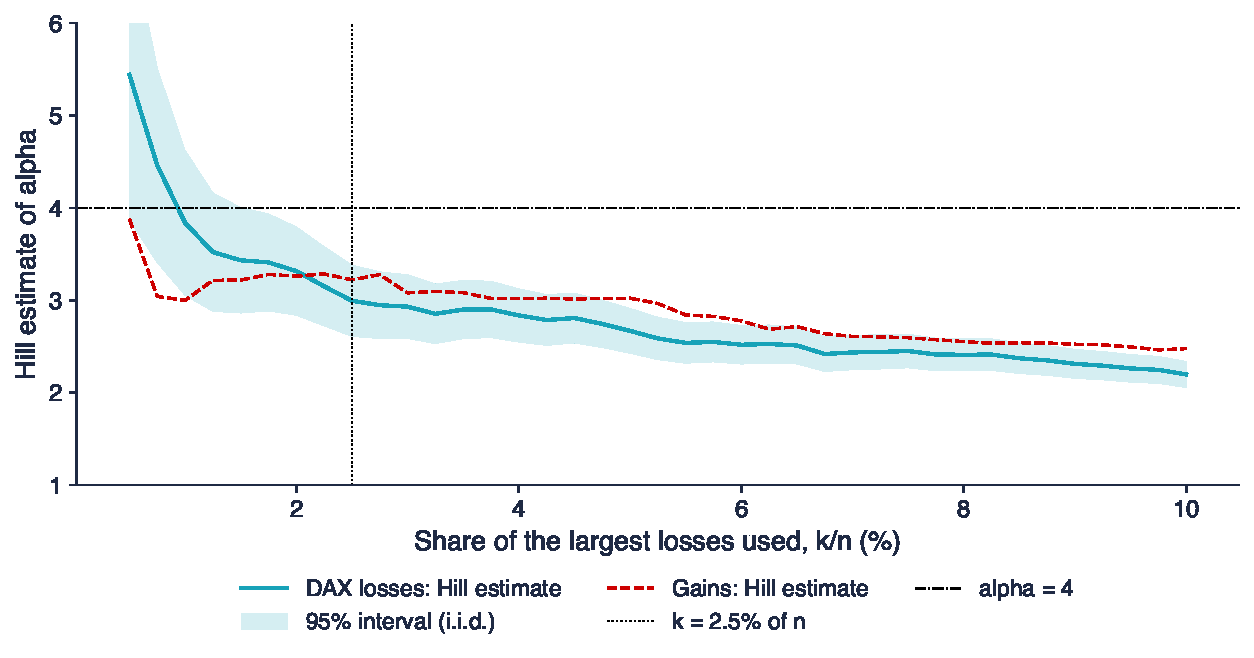
\includegraphics[width=0.96\textwidth,height=0.42\textheight,keepaspectratio]{ch5_sem_b1.pdf}
\end{center}
\vspace{-2mm}
\begin{itemize}
    \item $n = 9\,288$, $k = 232$, $L_{(k+1)} = 2.86\%$: $\hat\alpha = 3.00$, SE i.i.d.\ $0.20$, interval $[2.61, 3.38]$, SE block $0.20$; gains: $3.22$
    \item Between $k = 1\%$ and $5\%$ of $n$ the estimate falls slowly, from $3.84$ to $2.67$; the gains have a lighter tail
    \item Interpretation: $\alpha = 4$ is $-5.0$ block SE away: the kurtosis of DAX returns does not exist, so the sample kurtosis ($6.0$) is not a stable number
\end{itemize}\quantlet{SFM\_ch5\_seminar}{\qlurl{SFM_ch5_seminar}}
\end{frame}

\begin{frame}{B2: BET, Bitcoin and Two BVB Stocks [Proposed]}
\itemsize{\footnotesize}
\begin{itemize}
\item \textbf{Question}: which of the BET, Bitcoin, OMV Petrom and Banca Transilvania has the heaviest tail of losses? Model: B1.
\item \textbf{Inputs}: BET since 1997, Bitcoin since 2014, SNP and TLV since 2010 (TLV without 30--31 May 2016), daily losses in \%
\item \textbf{Tasks}
\begin{enumerate}
    \item Compute $\hat\alpha$ at $k = 2.5\%$ of $n$ for each series, with the 95\% interval and the block-bootstrap SE.
    \item Add the estimates at $k = 1\%$ and $5\%$ of $n$.
    \item Test the difference between the BET and Bitcoin with $z = (\hat\alpha_1 - \hat\alpha_2)/\sqrt{\mathrm{SE}_1^2 + \mathrm{SE}_2^2}$.
    \item Interpretation: is Bitcoin's tail heavier than the BET's once the scale of the losses is set aside?
\end{enumerate}
\item \textbf{Report}: one table, one $z$ and two sentences
\item Notebook: section B2
\end{itemize}
\end{frame}

\ifsolutions
\begin{frame}{B2: Solution [Proposed]}
\itemsize{\footnotesize}
\begin{center}
\footnotesize
\begin{tabular}{lrrrrrr}
\toprule
& $n$ & $k$ & $\hat\alpha$ & 95\% interval & SE block & $k = 1\%$ / $5\%$ \\
\midrule
BET & 7\,243 & 181 & $2.57$ & $[2.20, 2.95]$ & $0.23$ & $2.70$ / $2.16$ \\
Bitcoin & 4\,384 & 109 & $2.71$ & $[2.20, 3.21]$ & $0.23$ & $3.83$ / $2.49$ \\
OMV Petrom (SNP) & 3\,815 & 95 & $2.96$ & $[2.36, 3.56]$ & $0.39$ & $2.89$ / $2.60$ \\
Banca Transilvania (TLV) & 3\,788 & 94 & $2.49$ & $[1.98, 2.99]$ & $0.28$ & $3.05$ / $2.35$ \\
\bottomrule
\end{tabular}
\end{center}
\begin{itemize}
    \item BET vs Bitcoin: $z = -0.42$: no significant difference in the tail index
    \item All four estimates lie between $2.49$ and $2.96$; TLV has the lowest $\hat\alpha$, BET the second lowest
    \item Interpretation: Bitcoin's losses are much larger (the threshold $L_{(k+1)}$ is two to three times higher), but the shape of the tail is similar: scale and tail index are different things
\end{itemize}\quantlet{SFM\_ch5\_seminar}{\qlurl{SFM_ch5_seminar}}
\end{frame}
\fi

\begin{frame}{B3: POT for the BET [Solved]}
\itemsize{\scriptsize}
\begin{itemize}
\item \textbf{Question}: how large are VaR 1\%, ES 2.5\% and VaR 0.1\% of daily BET losses by EVT, compared with historical simulation and the Normal distribution?
\item \textbf{Inputs}: BET closes since 1997, daily losses in \%; $u$ = the 90\% quantile of the losses
\item \textbf{Tasks}
\begin{enumerate}
    \item Draw the empirical mean excess function and mark $u$.
    \item Fit a GPD to the excesses over $u$ by maximum likelihood; report $\hat\xi$ with its SE and $\hat\beta$.
    \item Draw the QQ plot of the excesses against the fitted GPD.
    \item Compute VaR 1\%, ES 2.5\% and VaR 0.1\% by EVT, by historical simulation and by the Normal distribution.
    \item Interpretation: which method would you use for the capital of a bank holding the BET, and why?
\end{enumerate}
\item \textbf{Report}: the two charts, a table of nine numbers and two sentences
\item Notebook: section B3
\end{itemize}
\end{frame}

\begin{frame}{B3: Solution [Solved]}
\itemsize{\scriptsize}
\begin{center}
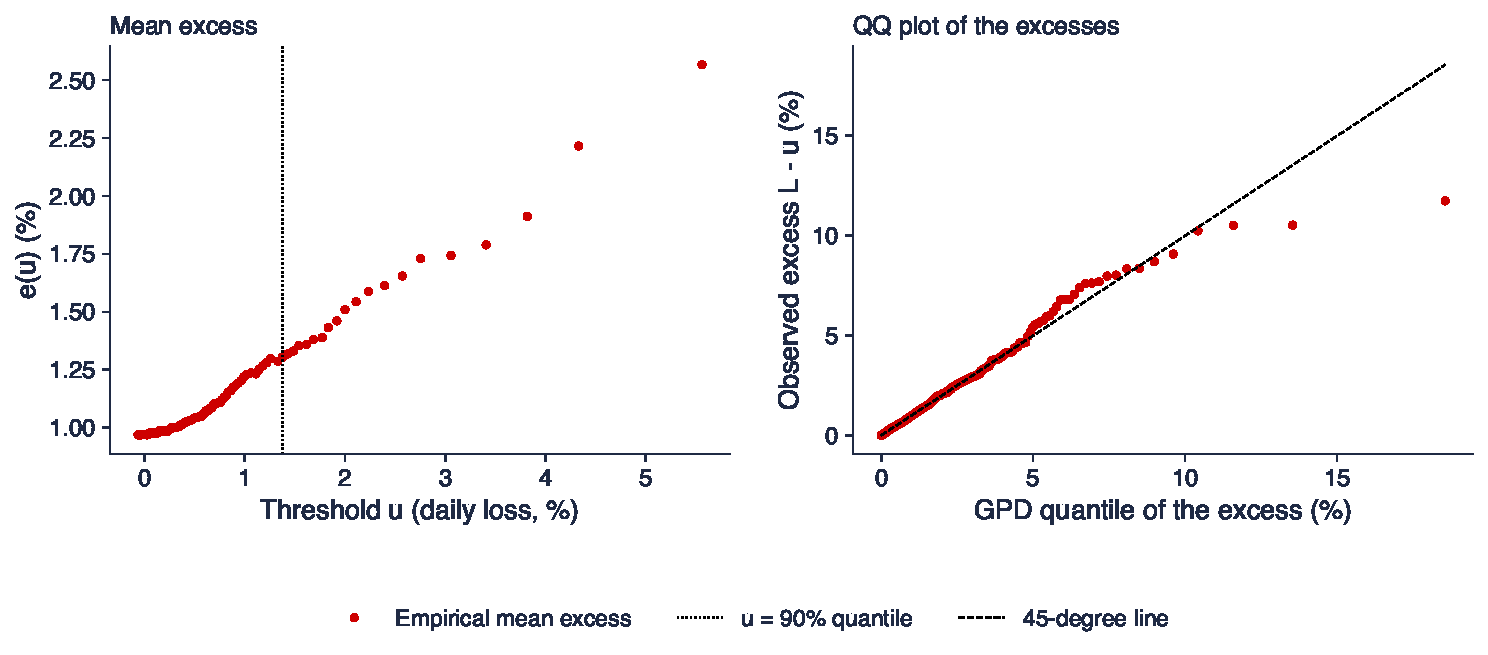
\includegraphics[width=0.96\textwidth,height=0.34\textheight,keepaspectratio]{ch5_sem_b3.pdf}
\end{center}
\vspace{-2mm}
\begin{center}
\scriptsize
\begin{tabular}{lrrr}
\toprule
(\%) & EVT & historical & Normal \\
\midrule
VaR 1\% & $4.44$ & $4.33$ & $3.39$ \\
ES 2.5\% & $4.81$ & $4.80$ & $3.41$ \\
VaR 0.1\% & $9.56$ & $9.64$ & $4.52$ \\
\bottomrule
\end{tabular}
\end{center}
\begin{itemize}
    \item $n = 7\,243$, $u = 1.375\%$, $N_u = 725$; $\hat\xi = 0.223$ (SE $0.047$), $\hat\beta = 1.018$; the mean excess rises linearly above $u$; the QQ plot is on the line except the largest excesses
    \item Interpretation: EVT, which agrees with the data at 1\% and gives a smooth VaR 0.1\%; the Normal VaR 0.1\% is less than half
\end{itemize}\quantlet{SFM\_ch5\_seminar}{\qlurl{SFM_ch5_seminar}}
\end{frame}

\begin{frame}{B4: Does the Threshold Matter? Bitcoin [Proposed]}
\itemsize{\footnotesize}
\begin{itemize}
\item \textbf{Question}: how much do $\hat\xi$ and the EVT risk measures of Bitcoin change with the threshold? Model: B3.
\item \textbf{Inputs}: Bitcoin since 2014, daily losses in \%; $u$ at the 85\%, 90\% and 95\% quantiles
\item \textbf{Tasks}
\begin{enumerate}
    \item For each threshold, fit the GPD and report $u$, $N_u$, $\hat\xi$ with its SE and $\hat\beta$.
    \item Compute VaR 1\%, ES 2.5\% and VaR 0.1\% for each threshold, and by historical simulation.
    \item Interpretation: which quantity is robust to the choice of $u$, $\hat\xi$ or the VaR?
\end{enumerate}
\item \textbf{Report}: one table and two sentences
\item Notebook: section B4
\end{itemize}
\end{frame}

\ifsolutions
\begin{frame}{B4: Solution [Proposed]}
\itemsize{\footnotesize}
\begin{center}
\footnotesize
\begin{tabular}{lrrrrrrr}
\toprule
$u$ at & $u$ (\%) & $N_u$ & $\hat\xi$ (SE) & $\hat\beta$ & VaR 1\% & ES 2.5\% & VaR 0.1\% \\
\midrule
85\% & $2.40$ & 658 & $0.15$ ($0.04$) & $2.37$ & $10.30$ & $10.90$ & $20.06$ \\
90\% & $3.33$ & 439 & $0.12$ ($0.05$) & $2.66$ & $10.38$ & $10.90$ & $19.61$ \\
95\% & $5.33$ & 220 & $0.16$ ($0.07$) & $2.65$ & $10.23$ & $10.84$ & $19.88$ \\
historical & & & & & $10.51$ & $10.84$ & $18.05$ \\
\bottomrule
\end{tabular}
\end{center}
\begin{itemize}
    \item $\hat\xi$ moves between thresholds by about one SE; the risk measures move by a few tenths of a percentage point only
    \item Interpretation: VaR and ES are robust to $u$ (the fit adjusts $\beta$); $\hat\xi$, and every extrapolation far beyond the data, is not
\end{itemize}\quantlet{SFM\_ch5\_seminar}{\qlurl{SFM_ch5_seminar}}
\end{frame}
\fi

\begin{frame}{B5: Quarterly Maxima of the S\&P 500 [Solved]}
\itemsize{\footnotesize}
\begin{itemize}
\item \textbf{Question}: how large is the daily loss that the S\&P 500 exceeds once in 10 years, according to a GEV fit to quarterly maxima?
\item \textbf{Inputs}: S\&P 500 closes since 1990, the largest daily loss of each calendar quarter
\item \textbf{Tasks}
\begin{enumerate}
    \item Build the quarterly maxima of the daily losses.
    \item Fit a GEV by maximum likelihood; report $\hat\xi$ with its 95\% interval, $\hat\mu$ and $\hat\sigma$.
    \item Draw the QQ plot and the return level plot.
    \item Compute the 10-year return level (40 quarters) and count the quarters above it.
    \item Interpretation: is the S\&P 500 tail Fréchet or Gumbel?
\end{enumerate}
\item \textbf{Report}: three parameters, one level, the charts and one sentence
\item Notebook: section B5
\end{itemize}
\end{frame}

\begin{frame}{B5: Solution [Solved]}
\itemsize{\footnotesize}
\begin{center}
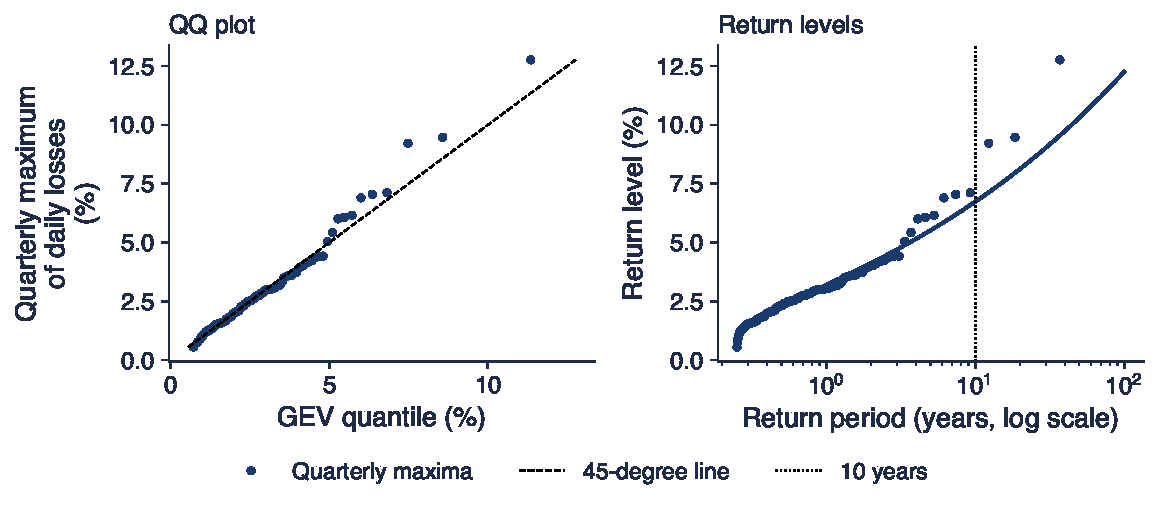
\includegraphics[width=0.96\textwidth,height=0.42\textheight,keepaspectratio]{ch5_sem_b5.pdf}
\end{center}
\vspace{-2mm}
\begin{itemize}
    \item 147 quarters: $\hat\xi = 0.21$, 95\% interval $[0.09, 0.32]$; $\hat\mu = 1.97\%$, $\hat\sigma = 0.86\%$
    \item 10-year return level: $6.7\%$; exceeded in 6 of 147 quarters ($3.7$ expected in 36.8 years); largest loss $12.8\%$
    \item Interpretation: $\xi = 0$ lies outside the interval: Fréchet, a heavy tail with $\alpha = 1/\hat\xi = 4.8$
\end{itemize}\quantlet{SFM\_ch5\_seminar}{\qlurl{SFM_ch5_seminar}}
\end{frame}

\begin{frame}{B6: Does VaR 1\% Survive a New Period? [Proposed]}
\itemsize{\footnotesize}
\begin{itemize}
\item \textbf{Question}: estimated until 2014, is the VaR 1\% of DAX and BET losses exceeded on about 1\% of the days of 2015--2026? Models: B3, B5.
\item \textbf{Inputs}: DAX since 1990, BET since 1997, daily losses in \%; estimation until 31 December 2014, test afterwards
\item \textbf{Tasks}
\begin{enumerate}
    \item Estimate VaR 1\% on the first period by EVT (POT, $u$ at the 90\% quantile), historical simulation and the Normal distribution.
    \item Count the test days with a loss above each VaR and compare with $np$.
    \item Compute the two-sided binomial p-value of each count.
    \item Interpretation: why can all three methods fail in the same direction?
\end{enumerate}
\item \textbf{Report}: a table with six counts and p-values, and two sentences
\item Notebook: section B6
\end{itemize}
\end{frame}

\ifsolutions
\begin{frame}{B6: Solution [Proposed]}
\itemsize{\footnotesize}
\begin{center}
\footnotesize
\begin{tabular}{lrrrrr}
\toprule
& test days & expected & EVT (p-value) & historical & Normal \\
\midrule
DAX & 2\,972 & $29.7$ & 14 ($0.002$) & 11 ($< 0.001$) & 36 ($0.288$) \\
BET & 2\,925 & $29.2$ & 8 ($< 0.001$) & 8 ($< 0.001$) & 13 ($0.001$) \\
\bottomrule
\end{tabular}
\end{center}
\begin{itemize}
    \item VaR 1\% (\%): DAX: EVT $4.12$, historical $4.32$, Normal $3.34$; BET: $5.07$, $5.13$, $3.99$
    \item EVT and historical: far fewer exceedances than expected (too conservative); the Normal VaR passes for the DAX by chance: a too-thin tail on a too-high variance
    \item Interpretation: 2015--2026 was calmer than 1990--2014; an unconditional VaR does not adapt to the volatility regime (\sfmchlink{https://danpele.github.io/SFM/EN/Courses/chapter9_arch_garch_models.pdf}{Chapters 9} and \sfmchlink{https://danpele.github.io/SFM/EN/Courses/chapter10_var_es_backtesting.pdf}{10})
\end{itemize}\quantlet{SFM\_ch5\_seminar}{\qlurl{SFM_ch5_seminar}}
\end{frame}
\fi


%=============================================================================
\section{Part C: Open Questions and AI Critique}
%=============================================================================

\begin{frame}{C1: Has the Tail of Bitcoin Changed? [Proposed]}
\itemsize{\footnotesize}
\begin{itemize}
\item \textbf{Question}: is the tail index of Bitcoin losses different in 2014--2017, 2018--2021 and 2022--2026?
\item \textbf{Inputs}: Bitcoin daily losses since 2014, split into three periods; models: B1, B2
\item \textbf{Tasks}
\begin{enumerate}
    \item Compute the Hill $\hat\alpha$ at $k = 2.5\%$ of $n$ in each period, with the block-bootstrap SE and a 95\% interval.
    \item Say whether any two periods differ significantly.
    \item Propose one change to the method that would give a sharper answer.
    \item Interpretation: what can a sample of about 1\,500 days say about a tail index?
\end{enumerate}
\item \textbf{Report}: a table, one sentence per comparison and a plan for a project
\item Notebook: section C1
\end{itemize}
\end{frame}

\ifsolutions
\begin{frame}{C1: Reference Analysis [Proposed]}
\itemsize{\footnotesize}
\begin{center}
\footnotesize
\begin{tabular}{lrrrrr}
\toprule
Period & $n$ & $k$ & $\hat\alpha$ & SE block & 95\% interval \\
\midrule
2014--2017 & 1201 & 30 & $2.68$ & $0.45$ & $[1.79, 3.57]$ \\
2018--2021 & 1461 & 36 & $3.23$ & $0.71$ & $[1.85, 4.62]$ \\
2022--2026 & 1722 & 43 & $2.88$ & $0.43$ & $[2.03, 3.74]$ \\
\bottomrule
\end{tabular}
\end{center}
\begin{itemize}
    \item All intervals overlap: no significant change; with $k$ between 30 and 43 the SE is $0.43$--$0.71$
    \item Sharper designs: GARCH-standardised losses (\sfmchlink{https://danpele.github.io/SFM/EN/Courses/chapter9_arch_garch_models.pdf}{Chapter 9}), POT with a common threshold, more crypto assets pooled, longer windows
    \item Interpretation: about 1\,500 days leave about 40 tail observations: enough for a rough $\alpha$, not for detecting a change of 0.5
\end{itemize}\quantlet{SFM\_ch5\_seminar}{\qlurl{SFM_ch5_seminar}}
\end{frame}
\fi

\begin{frame}{C2: Audit an AI Answer [Proposed]}
\itemsize{\scriptsize}
\begin{itemize}
    \item A student asked an AI assistant to estimate the tail of daily S\&P 500 losses since 1990 by POT. The answer:
    \item \aiprompt{(a) With u = 1.163\%, N\_u = 924 of n = 9\,240, the GPD gives xi = 0.158, so the tail index is alpha = 0.158 and the variance is infinite.}
    \item \aiprompt{(b) VaR 1\% = u + (beta/xi) [(n p / N\_u)\textasciicircum xi - 1] = -0.32\%.}
    \item \aiprompt{(c) ES 2.5\% = VaR 2.5\% x (1 - xi) = 1.98\%.}
    \item \aiprompt{(d) The same formula gives a reliable VaR 20\%.}
    \item \aiprompt{(e) Above u, the mean excess function of the fitted GPD is a straight line in the threshold.}
    \item Tasks
    \begin{itemize}
        \item 1. For each statement, say whether it is correct; if not, give the correct statement and, where possible, the correct number from the notebook (section C2).
        \item 2. Report: a list of five verdicts with one line of justification each.
    \end{itemize}
\end{itemize}
\end{frame}

\ifsolutions
\begin{frame}{C2: Solution [Proposed]}
\itemsize{\footnotesize}
\begin{itemize}
    \item (a) Wrong: $\alpha = 1/\xi = 6.3$, not $\xi$; the variance of a GPD tail is finite for $\xi < 1/2$
    \item (b) Wrong: the exponent is $-\xi$; VaR 1\% $= 3.30\%$ (a negative VaR, $-0.32\%$, below $u$, is a red flag)
    \item (c) Wrong: $\mathrm{ES}_p = (\mathrm{VaR}_p + \beta - \xi u)/(1 - \xi)$: VaR 2.5\% $= 2.35\%$, ES 2.5\% $= 3.49\%$; ES can never be below VaR
    \item (d) Wrong: the GPD models only the $N_u/n = 10\%$ largest losses; it is valid only for $p < 10\%$
    \item (e) Correct: $e(v) = (\beta + \xi(v - u))/(1 - \xi)$ for $v > u$, linear with slope $\xi/(1 - \xi)$
\end{itemize}\quantlet{SFM\_ch5\_seminar}{\qlurl{SFM_ch5_seminar}}
\end{frame}
\fi


%=============================================================================
\section{Wrap-Up}
%=============================================================================

\begin{frame}{What You Should Take from Today}
\itemsize{\small}
\begin{itemize}
    \item Daily losses have power tails with $\alpha$ between 2.5 and 3.5: finite variance, no finite kurtosis
    \item Hill: fix $k$ in a flat region of the Hill plot; report a standard error that allows for clustering
    \item POT: $u$ at a high quantile, GPD for the excesses, VaR and ES by closed formulas; check with mean excess and QQ plots
    \item Block maxima: GEV, Fréchet for financial losses; return levels beyond the sample are extrapolation
    \item An AI answer is a draft: check $\alpha = 1/\xi$, the sign of the exponent, ES $\ge$ VaR and the range $p < N_u/n$
\end{itemize}
\end{frame}

\begin{frame}{After the Seminar}
\itemsize{\small}
\begin{itemize}
    \item Lecture 5 develops each topic of today: crashes, regular variation, Hill, mean excess, GEV, GPD, EVT VaR and ES
    \item Try the [Proposed] tasks in the notebook; the solutions are discussed in class
    \item C1 can grow into a team project: GARCH-standardised losses, POT with a common threshold, more crypto assets
    \item Reading: \refFHH, Ch.~18; exercises in \refBHL, Ch.~18; \refQRM, Ch.~5
\end{itemize}
\end{frame}


%=============================================================================
\section{References}
%=============================================================================

\begin{frame}{References}
\itemsize{\tiny}
\begin{itemize}
    \item Balkema, A.A., de Haan, L. (1974). \href{https://doi.org/10.1214/aop/1176996548}{Residual life time at great age}. \textit{Annals of Probability}, 2(5), 792--804.
    \item Borak, S., Härdle, W.K., López-Cabrera, B. (2013). \href{https://doi.org/10.1007/978-3-642-33929-5}{\textit{Statistics of Financial Markets: Exercises and Solutions}}, 2nd ed. Springer.
    \item Fisher, R.A., Tippett, L.H.C. (1928). \href{https://doi.org/10.1017/S0305004100015681}{Limiting forms of the frequency distribution of the largest or smallest member of a sample}. \textit{Mathematical Proceedings of the Cambridge Philosophical Society}, 24(2), 180--190.
    \item Franke, J., Härdle, W.K., Hafner, C.M. (2019). \href{https://doi.org/10.1007/978-3-030-13751-9}{\textit{Statistics of Financial Markets: An Introduction}}, 5th ed. Springer.
    \item Gnedenko, B. (1943). \href{https://doi.org/10.2307/1968974}{Sur la distribution limite du terme maximum d'une série aléatoire}. \textit{Annals of Mathematics}, 44(3), 423--453.
    \item Hill, B.M. (1975). \href{https://doi.org/10.1214/aos/1176343247}{A simple general approach to inference about the tail of a distribution}. \textit{Annals of Statistics}, 3(5), 1163--1174.
    \item McNeil, A.J., Frey, R. (2000). \href{https://doi.org/10.1016/S0927-5398(00)00012-8}{Estimation of tail-related risk measures for heteroscedastic financial time series: an extreme value approach}. \textit{Journal of Empirical Finance}, 7(3--4), 271--300.
    \item McNeil, A.J., Frey, R., Embrechts, P. (2015). \href{https://press.princeton.edu/books/hardcover/9780691166278/quantitative-risk-management}{\textit{Quantitative Risk Management: Concepts, Techniques and Tools}}, revised ed. Princeton University Press.
    \item Pickands, J. (1975). \href{https://doi.org/10.1214/aos/1176343003}{Statistical inference using extreme order statistics}. \textit{Annals of Statistics}, 3(1), 119--131.
    \item Weissman, I. (1978). \href{https://doi.org/10.1080/01621459.1978.10480104}{Estimation of parameters and large quantiles based on the $k$ largest observations}. \textit{Journal of the American Statistical Association}, 73(364), 812--815.
\end{itemize}
\end{frame}

\end{document}
